\documentclass[twoside]{book}

% Packages required by doxygen
\usepackage{fixltx2e}
\usepackage{calc}
\usepackage{doxygen}
\usepackage[export]{adjustbox} % also loads graphicx
\usepackage{graphicx}
\usepackage[utf8]{inputenc}
\usepackage{makeidx}
\usepackage{multicol}
\usepackage{multirow}
\PassOptionsToPackage{warn}{textcomp}
\usepackage{textcomp}
\usepackage[nointegrals]{wasysym}
\usepackage[table]{xcolor}

% Font selection
\usepackage[T1]{fontenc}
\usepackage[scaled=.90]{helvet}
\usepackage{courier}
\usepackage{amssymb}
\usepackage{sectsty}
\renewcommand{\familydefault}{\sfdefault}
\allsectionsfont{%
  \fontseries{bc}\selectfont%
  \color{darkgray}%
}
\renewcommand{\DoxyLabelFont}{%
  \fontseries{bc}\selectfont%
  \color{darkgray}%
}
\newcommand{\+}{\discretionary{\mbox{\scriptsize$\hookleftarrow$}}{}{}}

% Page & text layout
\usepackage{geometry}
\geometry{%
  a4paper,%
  top=2.5cm,%
  bottom=2.5cm,%
  left=2.5cm,%
  right=2.5cm%
}
\tolerance=750
\hfuzz=15pt
\hbadness=750
\setlength{\emergencystretch}{15pt}
\setlength{\parindent}{0cm}
\setlength{\parskip}{3ex plus 2ex minus 2ex}
\makeatletter
\renewcommand{\paragraph}{%
  \@startsection{paragraph}{4}{0ex}{-1.0ex}{1.0ex}{%
    \normalfont\normalsize\bfseries\SS@parafont%
  }%
}
\renewcommand{\subparagraph}{%
  \@startsection{subparagraph}{5}{0ex}{-1.0ex}{1.0ex}{%
    \normalfont\normalsize\bfseries\SS@subparafont%
  }%
}
\makeatother

% Headers & footers
\usepackage{fancyhdr}
\pagestyle{fancyplain}
\fancyhead[LE]{\fancyplain{}{\bfseries\thepage}}
\fancyhead[CE]{\fancyplain{}{}}
\fancyhead[RE]{\fancyplain{}{\bfseries\leftmark}}
\fancyhead[LO]{\fancyplain{}{\bfseries\rightmark}}
\fancyhead[CO]{\fancyplain{}{}}
\fancyhead[RO]{\fancyplain{}{\bfseries\thepage}}
\fancyfoot[LE]{\fancyplain{}{}}
\fancyfoot[CE]{\fancyplain{}{}}
\fancyfoot[RE]{\fancyplain{}{\bfseries\scriptsize Generated by Doxygen }}
\fancyfoot[LO]{\fancyplain{}{\bfseries\scriptsize Generated by Doxygen }}
\fancyfoot[CO]{\fancyplain{}{}}
\fancyfoot[RO]{\fancyplain{}{}}
\renewcommand{\footrulewidth}{0.4pt}
\renewcommand{\chaptermark}[1]{%
  \markboth{#1}{}%
}
\renewcommand{\sectionmark}[1]{%
  \markright{\thesection\ #1}%
}

% Indices & bibliography
\usepackage{natbib}
\usepackage[titles]{tocloft}
\setcounter{tocdepth}{3}
\setcounter{secnumdepth}{5}
\makeindex

% Hyperlinks (required, but should be loaded last)
\usepackage{ifpdf}
\ifpdf
  \usepackage[pdftex,pagebackref=true]{hyperref}
\else
  \usepackage[ps2pdf,pagebackref=true]{hyperref}
\fi
\hypersetup{%
  colorlinks=true,%
  linkcolor=blue,%
  citecolor=blue,%
  unicode%
}

% Custom commands
\newcommand{\clearemptydoublepage}{%
  \newpage{\pagestyle{empty}\cleardoublepage}%
}

\usepackage{caption}
\captionsetup{labelsep=space,justification=centering,font={bf},singlelinecheck=off,skip=4pt,position=top}

%===== C O N T E N T S =====

\begin{document}

% Titlepage & ToC
\hypersetup{pageanchor=false,
             bookmarksnumbered=true,
             pdfencoding=unicode
            }
\pagenumbering{alph}
\begin{titlepage}
\vspace*{7cm}
\begin{center}%
{\Large bfjit \\[1ex]\large 0.\+1 }\\
\vspace*{1cm}
{\large Generated by Doxygen 1.8.12}\\
\end{center}
\end{titlepage}
\clearemptydoublepage
\pagenumbering{roman}
\tableofcontents
\clearemptydoublepage
\pagenumbering{arabic}
\hypersetup{pageanchor=true}

%--- Begin generated contents ---
\chapter{R\+E\+A\+D\+ME}
\label{md_README}
\hypertarget{md_README}{}
\input{md_README}
\chapter{Namespace Index}
\section{Namespace List}
Here is a list of all documented namespaces with brief descriptions\+:\begin{DoxyCompactList}
\item\contentsline{section}{\hyperlink{namespacebfjit}{bfjit} \\*Namespace that contains all bfjit-\/related classes and functions }{\pageref{namespacebfjit}}{}
\end{DoxyCompactList}

\chapter{Hierarchical Index}
\section{Class Hierarchy}
This inheritance list is sorted roughly, but not completely, alphabetically\+:\begin{DoxyCompactList}
\item \contentsline{section}{bfjit\+:\+:ast}{\pageref{classbfjit_1_1ast}}{}
\begin{DoxyCompactList}
\item \contentsline{section}{bfjit\+:\+:io\+\_\+ast}{\pageref{classbfjit_1_1io__ast}}{}
\item \contentsline{section}{bfjit\+:\+:loop\+\_\+ast}{\pageref{classbfjit_1_1loop__ast}}{}
\item \contentsline{section}{bfjit\+:\+:movement\+\_\+ast}{\pageref{classbfjit_1_1movement__ast}}{}
\item \contentsline{section}{bfjit\+:\+:mutation\+\_\+ast}{\pageref{classbfjit_1_1mutation__ast}}{}
\end{DoxyCompactList}
\item \contentsline{section}{bfjit\+:\+:jit\+\_\+function}{\pageref{classbfjit_1_1jit__function}}{}
\item \contentsline{section}{options}{\pageref{structoptions}}{}
\item \contentsline{section}{bfjit\+:\+:parse\+\_\+error}{\pageref{classbfjit_1_1parse__error}}{}
\item \contentsline{section}{bfjit\+:\+:position}{\pageref{classbfjit_1_1position}}{}
\item \contentsline{section}{bfjit\+:\+:token}{\pageref{classbfjit_1_1token}}{}
\end{DoxyCompactList}

\chapter{Class Index}
\section{Class List}
Here are the classes, structs, unions and interfaces with brief descriptions\+:\begin{DoxyCompactList}
\item\contentsline{section}{\hyperlink{classbfjit_1_1ast}{bfjit\+::ast} \\*Abstract base class of all other ast classes }{\pageref{classbfjit_1_1ast}}{}
\item\contentsline{section}{\hyperlink{classbfjit_1_1io__ast}{bfjit\+::io\+\_\+ast} \\*A class that represent a single I/O instruction }{\pageref{classbfjit_1_1io__ast}}{}
\item\contentsline{section}{\hyperlink{classbfjit_1_1jit__function}{bfjit\+::jit\+\_\+function} \\*A class that represents code ready for execution }{\pageref{classbfjit_1_1jit__function}}{}
\item\contentsline{section}{\hyperlink{classbfjit_1_1loop__ast}{bfjit\+::loop\+\_\+ast} \\*A class that represents a brainfuck loop }{\pageref{classbfjit_1_1loop__ast}}{}
\item\contentsline{section}{\hyperlink{classbfjit_1_1movement__ast}{bfjit\+::movement\+\_\+ast} \\*A class that represents a movement instruction }{\pageref{classbfjit_1_1movement__ast}}{}
\item\contentsline{section}{\hyperlink{classbfjit_1_1mutation__ast}{bfjit\+::mutation\+\_\+ast} \\*A class that represents a single (cellmutation) instruction }{\pageref{classbfjit_1_1mutation__ast}}{}
\item\contentsline{section}{\hyperlink{structoptions}{options} }{\pageref{structoptions}}{}
\item\contentsline{section}{\hyperlink{classbfjit_1_1parse__error}{bfjit\+::parse\+\_\+error} }{\pageref{classbfjit_1_1parse__error}}{}
\item\contentsline{section}{\hyperlink{classbfjit_1_1position}{bfjit\+::position} \\*A class that tracks position of a token in a stream }{\pageref{classbfjit_1_1position}}{}
\item\contentsline{section}{\hyperlink{classbfjit_1_1token}{bfjit\+::token} \\*A class that represents a single token extracted from a stream }{\pageref{classbfjit_1_1token}}{}
\end{DoxyCompactList}

\chapter{Namespace Documentation}
\hypertarget{namespacebfjit}{}\section{bfjit Namespace Reference}
\label{namespacebfjit}\index{bfjit@{bfjit}}


Namespace that contains all bfjit-\/related classes and functions.  


\subsection*{Classes}
\begin{DoxyCompactItemize}
\item 
class \hyperlink{classbfjit_1_1ast}{ast}
\begin{DoxyCompactList}\small\item\em Abstract base class of all other ast classes. \end{DoxyCompactList}\item 
class \hyperlink{classbfjit_1_1io__ast}{io\+\_\+ast}
\begin{DoxyCompactList}\small\item\em A class that represent a single I/O instruction. \end{DoxyCompactList}\item 
class \hyperlink{classbfjit_1_1jit__function}{jit\+\_\+function}
\begin{DoxyCompactList}\small\item\em A class that represents code ready for execution. \end{DoxyCompactList}\item 
class \hyperlink{classbfjit_1_1loop__ast}{loop\+\_\+ast}
\begin{DoxyCompactList}\small\item\em A class that represents a brainfuck loop. \end{DoxyCompactList}\item 
class \hyperlink{classbfjit_1_1movement__ast}{movement\+\_\+ast}
\begin{DoxyCompactList}\small\item\em A class that represents a movement instruction. \end{DoxyCompactList}\item 
class \hyperlink{classbfjit_1_1mutation__ast}{mutation\+\_\+ast}
\begin{DoxyCompactList}\small\item\em A class that represents a single (cellmutation) instruction. \end{DoxyCompactList}\item 
class \hyperlink{classbfjit_1_1parse__error}{parse\+\_\+error}
\item 
class \hyperlink{classbfjit_1_1position}{position}
\begin{DoxyCompactList}\small\item\em A class that tracks position of a token in a stream. \end{DoxyCompactList}\item 
class \hyperlink{classbfjit_1_1token}{token}
\begin{DoxyCompactList}\small\item\em A class that represents a single token extracted from a stream. \end{DoxyCompactList}\end{DoxyCompactItemize}
\subsection*{Typedefs}
\begin{DoxyCompactItemize}
\item 
\hypertarget{namespacebfjit_ad9bbdb76861e57928b1bc7695c2c0623}{}\label{namespacebfjit_ad9bbdb76861e57928b1bc7695c2c0623} 
using \hyperlink{namespacebfjit_ad9bbdb76861e57928b1bc7695c2c0623}{combined\+\_\+ast} = mapbox\+::util\+::variant$<$ \hyperlink{classbfjit_1_1movement__ast}{movement\+\_\+ast}, \hyperlink{classbfjit_1_1mutation__ast}{mutation\+\_\+ast}, \hyperlink{classbfjit_1_1io__ast}{io\+\_\+ast}, mapbox\+::util\+::recursive\+\_\+wrapper$<$ \hyperlink{classbfjit_1_1loop__ast}{loop\+\_\+ast} $>$$>$
\begin{DoxyCompactList}\small\item\em A typedef that unites all ast types into a single variant. \end{DoxyCompactList}\item 
using \hyperlink{namespacebfjit_ac770ef0753b4d7d6bd5800262ba97f25}{parse\+\_\+result} = mapbox\+::util\+::variant$<$ \hyperlink{classbfjit_1_1parse__error}{parse\+\_\+error}, std\+::vector$<$ \hyperlink{namespacebfjit_ad9bbdb76861e57928b1bc7695c2c0623}{combined\+\_\+ast} $>$ $>$
\begin{DoxyCompactList}\small\item\em A typedef that represents the parsing result. \end{DoxyCompactList}\end{DoxyCompactItemize}
\subsection*{Functions}
\begin{DoxyCompactItemize}
\item 
\hypertarget{namespacebfjit_ab8c637e2dc36f385821956bc174d4030}{}\label{namespacebfjit_ab8c637e2dc36f385821956bc174d4030} 
std\+::ostream \& \hyperlink{namespacebfjit_ab8c637e2dc36f385821956bc174d4030}{operator$<$$<$} (std\+::ostream \&out, const \hyperlink{classbfjit_1_1movement__ast_a3aa723a03d76c31e1e88be817670701f}{movement\+\_\+ast\+::type} \&ty)
\begin{DoxyCompactList}\small\item\em A function that pretty-\/prints a \hyperlink{classbfjit_1_1movement__ast_a3aa723a03d76c31e1e88be817670701f}{movement\+\_\+ast\+::type} object. \end{DoxyCompactList}\item 
\hypertarget{namespacebfjit_ae08ef2d872d3d9132f0c721fa8489178}{}\label{namespacebfjit_ae08ef2d872d3d9132f0c721fa8489178} 
std\+::ostream \& \hyperlink{namespacebfjit_ae08ef2d872d3d9132f0c721fa8489178}{operator$<$$<$} (std\+::ostream \&out, const \hyperlink{classbfjit_1_1movement__ast}{movement\+\_\+ast} \&mast)
\begin{DoxyCompactList}\small\item\em A function that pretty-\/prints a \hyperlink{classbfjit_1_1token}{token} object. \end{DoxyCompactList}\item 
\hypertarget{namespacebfjit_ae267e9d951306b902f07d1c72413e58d}{}\label{namespacebfjit_ae267e9d951306b902f07d1c72413e58d} 
std\+::ostream \& \hyperlink{namespacebfjit_ae267e9d951306b902f07d1c72413e58d}{operator$<$$<$} (std\+::ostream \&out, const \hyperlink{classbfjit_1_1mutation__ast_a4a35ab616dab7944deedac4300f473e9}{mutation\+\_\+ast\+::type} \&ty)
\begin{DoxyCompactList}\small\item\em A function that pretty-\/prints a \hyperlink{classbfjit_1_1mutation__ast_a4a35ab616dab7944deedac4300f473e9}{mutation\+\_\+ast\+::type} object. \end{DoxyCompactList}\item 
\hypertarget{namespacebfjit_a5cb30f43ec85193cfda8b2169d776527}{}\label{namespacebfjit_a5cb30f43ec85193cfda8b2169d776527} 
std\+::ostream \& \hyperlink{namespacebfjit_a5cb30f43ec85193cfda8b2169d776527}{operator$<$$<$} (std\+::ostream \&out, const \hyperlink{classbfjit_1_1mutation__ast}{mutation\+\_\+ast} \&mast)
\begin{DoxyCompactList}\small\item\em A function that pretty-\/prints a \hyperlink{classbfjit_1_1mutation__ast}{mutation\+\_\+ast} object. \end{DoxyCompactList}\item 
\hypertarget{namespacebfjit_a51292e2e92a0bbf2bc1930d5437693e0}{}\label{namespacebfjit_a51292e2e92a0bbf2bc1930d5437693e0} 
std\+::ostream \& \hyperlink{namespacebfjit_a51292e2e92a0bbf2bc1930d5437693e0}{operator$<$$<$} (std\+::ostream \&out, const \hyperlink{classbfjit_1_1io__ast_ae0b93ddde6f86aed45dd22b72d290414}{io\+\_\+ast\+::type} \&ty)
\begin{DoxyCompactList}\small\item\em A function that pretty-\/prints a \hyperlink{classbfjit_1_1io__ast_ae0b93ddde6f86aed45dd22b72d290414}{io\+\_\+ast\+::type} object. \end{DoxyCompactList}\item 
\hypertarget{namespacebfjit_af52c593484b4d6f0fe4febf43811b027}{}\label{namespacebfjit_af52c593484b4d6f0fe4febf43811b027} 
std\+::ostream \& \hyperlink{namespacebfjit_af52c593484b4d6f0fe4febf43811b027}{operator$<$$<$} (std\+::ostream \&out, const \hyperlink{classbfjit_1_1io__ast}{io\+\_\+ast} \&ioast)
\begin{DoxyCompactList}\small\item\em A function that pretty-\/prints a \hyperlink{classbfjit_1_1io__ast}{io\+\_\+ast} object. \end{DoxyCompactList}\item 
\hypertarget{namespacebfjit_a845e544a129fbae6cd93460021922bea}{}\label{namespacebfjit_a845e544a129fbae6cd93460021922bea} 
std\+::ostream \& \hyperlink{namespacebfjit_a845e544a129fbae6cd93460021922bea}{operator$<$$<$} (std\+::ostream \&out, const \hyperlink{classbfjit_1_1loop__ast}{loop\+\_\+ast} \&ioast)
\begin{DoxyCompactList}\small\item\em A function that pretty-\/prints a \hyperlink{classbfjit_1_1loop__ast}{loop\+\_\+ast} object. \end{DoxyCompactList}\item 
\hypertarget{namespacebfjit_ae0af2cb10b3785b75f51e846b46fbc00}{}\label{namespacebfjit_ae0af2cb10b3785b75f51e846b46fbc00} 
void {\bfseries prologue} (jit\+\_\+function\+::impl $\ast$impl)
\item 
\hypertarget{namespacebfjit_aa8e79a40d19e72d22ade985a63055392}{}\label{namespacebfjit_aa8e79a40d19e72d22ade985a63055392} 
void {\bfseries epilogue} (jit\+\_\+function\+::impl $\ast$impl)
\item 
\hypertarget{namespacebfjit_a2074dd9fc2ff8ea0960e66bdb2bb9a5a}{}\label{namespacebfjit_a2074dd9fc2ff8ea0960e66bdb2bb9a5a} 
void {\bfseries movement} (jit\+\_\+function\+::impl $\ast$impl, const \hyperlink{classbfjit_1_1movement__ast}{movement\+\_\+ast} \&m\+\_\+ast)
\item 
\hypertarget{namespacebfjit_a73bb08eeefd210b9252ae57d5e920956}{}\label{namespacebfjit_a73bb08eeefd210b9252ae57d5e920956} 
void {\bfseries mutation} (jit\+\_\+function\+::impl $\ast$impl, const \hyperlink{classbfjit_1_1mutation__ast}{mutation\+\_\+ast} \&m\+\_\+ast)
\item 
\hypertarget{namespacebfjit_af8ac98f27907450e44251e60653b8226}{}\label{namespacebfjit_af8ac98f27907450e44251e60653b8226} 
void {\bfseries io} (jit\+\_\+function\+::impl $\ast$impl, const \hyperlink{classbfjit_1_1io__ast}{io\+\_\+ast} \&i\+\_\+ast)
\item 
\hypertarget{namespacebfjit_a0cca116c9c12075bcd8866d50251327d}{}\label{namespacebfjit_a0cca116c9c12075bcd8866d50251327d} 
void {\bfseries loop} (jit\+\_\+function\+::impl $\ast$impl, const \hyperlink{classbfjit_1_1loop__ast}{loop\+\_\+ast} \&l\+\_\+ast)
\item 
std\+::vector$<$ \hyperlink{classbfjit_1_1token}{token} $>$ \hyperlink{namespacebfjit_afc8d63bb8e810f0a8386783924340045}{lex} (std\+::istream \&stream)
\begin{DoxyCompactList}\small\item\em A function that reads \hyperlink{classbfjit_1_1token}{token}s from a stream. \end{DoxyCompactList}\item 
std\+::vector$<$ \hyperlink{namespacebfjit_ad9bbdb76861e57928b1bc7695c2c0623}{combined\+\_\+ast} $>$ \hyperlink{namespacebfjit_a6d6a3107cfe22399215c398dd5d25d85}{optimize} (std\+::vector$<$ \hyperlink{namespacebfjit_ad9bbdb76861e57928b1bc7695c2c0623}{combined\+\_\+ast} $>$\+::const\+\_\+iterator begin\+\_\+it, std\+::vector$<$ \hyperlink{namespacebfjit_ad9bbdb76861e57928b1bc7695c2c0623}{combined\+\_\+ast} $>$\+::const\+\_\+iterator end\+\_\+it)
\begin{DoxyCompactList}\small\item\em Optimizes the input \hyperlink{namespacebfjit_ad9bbdb76861e57928b1bc7695c2c0623}{combined\+\_\+ast}\%. \end{DoxyCompactList}\item 
\hypertarget{namespacebfjit_ae336474650e07d599dae9e197f7565a2}{}\label{namespacebfjit_ae336474650e07d599dae9e197f7565a2} 
std\+::ostream \& \hyperlink{namespacebfjit_ae336474650e07d599dae9e197f7565a2}{operator$<$$<$} (std\+::ostream \&out, const \hyperlink{classbfjit_1_1parse__error_af750138d196890dcdc543c9fb1b7705b}{parse\+\_\+error\+::type} \&ty)
\begin{DoxyCompactList}\small\item\em A function that pretty-\/prints a \hyperlink{classbfjit_1_1parse__error_af750138d196890dcdc543c9fb1b7705b}{parse\+\_\+error\+::type} object. \end{DoxyCompactList}\item 
\hypertarget{namespacebfjit_a06209a97706aaee7244404eabb4a1399}{}\label{namespacebfjit_a06209a97706aaee7244404eabb4a1399} 
std\+::ostream \& \hyperlink{namespacebfjit_a06209a97706aaee7244404eabb4a1399}{operator$<$$<$} (std\+::ostream \&out, const \hyperlink{classbfjit_1_1parse__error}{parse\+\_\+error} \&pe)
\begin{DoxyCompactList}\small\item\em A function that pretty-\/prints a \hyperlink{classbfjit_1_1parse__error}{parse\+\_\+error} object. \end{DoxyCompactList}\item 
\hyperlink{namespacebfjit_ac770ef0753b4d7d6bd5800262ba97f25}{parse\+\_\+result} \hyperlink{namespacebfjit_add88f8f5cb8f1e6fe6d1ab62b2d5b9b4}{parse} (std\+::vector$<$ \hyperlink{classbfjit_1_1token}{token} $>$\+::const\+\_\+iterator begin\+\_\+it, std\+::vector$<$ \hyperlink{classbfjit_1_1token}{token} $>$\+::const\+\_\+iterator end\+\_\+it)
\begin{DoxyCompactList}\small\item\em A function that parses tokens into ast. \end{DoxyCompactList}\item 
\hypertarget{namespacebfjit_a339fdcb6eed0bc209bbf18598cbd4084}{}\label{namespacebfjit_a339fdcb6eed0bc209bbf18598cbd4084} 
std\+::ostream \& \hyperlink{namespacebfjit_a339fdcb6eed0bc209bbf18598cbd4084}{operator$<$$<$} (std\+::ostream \&out, const \hyperlink{classbfjit_1_1position}{position} \&p)
\begin{DoxyCompactList}\small\item\em A functions that pretty-\/prints a \hyperlink{classbfjit_1_1position}{position} object to a stream. \end{DoxyCompactList}\item 
\hypertarget{namespacebfjit_a5d7d8fa478e49f0143fc57fc6e28ffba}{}\label{namespacebfjit_a5d7d8fa478e49f0143fc57fc6e28ffba} 
std\+::ostream \& \hyperlink{namespacebfjit_a5d7d8fa478e49f0143fc57fc6e28ffba}{operator$<$$<$} (std\+::ostream \&out, const \hyperlink{classbfjit_1_1token_a2486a3e583fb48f3863c4eb5c32cdd96}{token\+::type} \&ty)
\begin{DoxyCompactList}\small\item\em A function that pretty-\/prints a \hyperlink{classbfjit_1_1token_a2486a3e583fb48f3863c4eb5c32cdd96}{token\+::type} object. \end{DoxyCompactList}\item 
\hypertarget{namespacebfjit_aa0300e35ddafd8014da5627a332ad3a9}{}\label{namespacebfjit_aa0300e35ddafd8014da5627a332ad3a9} 
std\+::ostream \& \hyperlink{namespacebfjit_aa0300e35ddafd8014da5627a332ad3a9}{operator$<$$<$} (std\+::ostream \&out, const \hyperlink{classbfjit_1_1token}{token} \&tok)
\begin{DoxyCompactList}\small\item\em A function that pretty-\/prints a \hyperlink{classbfjit_1_1token}{token} object. \end{DoxyCompactList}\item 
\hypertarget{namespacebfjit_a99ffba753326db1168413603b2ad07c5}{}\label{namespacebfjit_a99ffba753326db1168413603b2ad07c5} 
vector$<$ \hyperlink{classbfjit_1_1token}{token} $>$\+::const\+\_\+iterator {\bfseries parse\+\_\+helper} (vector$<$ \hyperlink{classbfjit_1_1token}{token} $>$\+::const\+\_\+iterator begin\+\_\+it, vector$<$ \hyperlink{classbfjit_1_1token}{token} $>$\+::const\+\_\+iterator end\+\_\+it, vector$<$ \hyperlink{namespacebfjit_ad9bbdb76861e57928b1bc7695c2c0623}{combined\+\_\+ast} $>$ \&vast)
\end{DoxyCompactItemize}


\subsection{Detailed Description}
Namespace that contains all bfjit-\/related classes and functions. 

\subsection{Typedef Documentation}
\hypertarget{namespacebfjit_ac770ef0753b4d7d6bd5800262ba97f25}{}\label{namespacebfjit_ac770ef0753b4d7d6bd5800262ba97f25} 
\index{bfjit@{bfjit}!parse\+\_\+result@{parse\+\_\+result}}
\index{parse\+\_\+result@{parse\+\_\+result}!bfjit@{bfjit}}
\subsubsection{\texorpdfstring{parse\+\_\+result}{parse\_result}}
{\footnotesize\ttfamily using \hyperlink{namespacebfjit_ac770ef0753b4d7d6bd5800262ba97f25}{bfjit\+::parse\+\_\+result} = typedef mapbox\+::util\+::variant $<$ \hyperlink{classbfjit_1_1parse__error}{parse\+\_\+error} , std\+::vector$<$\hyperlink{namespacebfjit_ad9bbdb76861e57928b1bc7695c2c0623}{combined\+\_\+ast}$>$ $>$}



A typedef that represents the parsing result. 

If parsing fails, the variant is set to an appropriate error message. If the parsing fails, the variant is set to a vector containing the ast. 

\subsection{Function Documentation}
\hypertarget{namespacebfjit_afc8d63bb8e810f0a8386783924340045}{}\label{namespacebfjit_afc8d63bb8e810f0a8386783924340045} 
\index{bfjit@{bfjit}!lex@{lex}}
\index{lex@{lex}!bfjit@{bfjit}}
\subsubsection{\texorpdfstring{lex()}{lex()}}
{\footnotesize\ttfamily vector$<$ \hyperlink{classbfjit_1_1token}{token} $>$ bfjit\+::lex (\begin{DoxyParamCaption}\item[{std\+::istream \&}]{stream }\end{DoxyParamCaption})}



A function that reads \hyperlink{classbfjit_1_1token}{token}s from a stream. 


\begin{DoxyParams}{Parameters}
{\em stream} & The stream to read. \\
\hline
\end{DoxyParams}
\hypertarget{namespacebfjit_a6d6a3107cfe22399215c398dd5d25d85}{}\label{namespacebfjit_a6d6a3107cfe22399215c398dd5d25d85} 
\index{bfjit@{bfjit}!optimize@{optimize}}
\index{optimize@{optimize}!bfjit@{bfjit}}
\subsubsection{\texorpdfstring{optimize()}{optimize()}}
{\footnotesize\ttfamily vector$<$ \hyperlink{namespacebfjit_ad9bbdb76861e57928b1bc7695c2c0623}{combined\+\_\+ast} $>$ bfjit\+::optimize (\begin{DoxyParamCaption}\item[{std\+::vector$<$ \hyperlink{namespacebfjit_ad9bbdb76861e57928b1bc7695c2c0623}{combined\+\_\+ast} $>$\+::const\+\_\+iterator}]{begin\+\_\+it,  }\item[{std\+::vector$<$ \hyperlink{namespacebfjit_ad9bbdb76861e57928b1bc7695c2c0623}{combined\+\_\+ast} $>$\+::const\+\_\+iterator}]{end\+\_\+it }\end{DoxyParamCaption})}



Optimizes the input \hyperlink{namespacebfjit_ad9bbdb76861e57928b1bc7695c2c0623}{combined\+\_\+ast}\%. 


\begin{DoxyParams}{Parameters}
{\em begin\+\_\+it} & An iterator to the beginning of ast to be optimized. \\
\hline
{\em end\+\_\+it} & An iterator to the end of ast to be optimized. \\
\hline
\end{DoxyParams}
\hypertarget{namespacebfjit_add88f8f5cb8f1e6fe6d1ab62b2d5b9b4}{}\label{namespacebfjit_add88f8f5cb8f1e6fe6d1ab62b2d5b9b4} 
\index{bfjit@{bfjit}!parse@{parse}}
\index{parse@{parse}!bfjit@{bfjit}}
\subsubsection{\texorpdfstring{parse()}{parse()}}
{\footnotesize\ttfamily \hyperlink{namespacebfjit_ac770ef0753b4d7d6bd5800262ba97f25}{parse\+\_\+result} bfjit\+::parse (\begin{DoxyParamCaption}\item[{std\+::vector$<$ \hyperlink{classbfjit_1_1token}{token} $>$\+::const\+\_\+iterator}]{begin\+\_\+it,  }\item[{std\+::vector$<$ \hyperlink{classbfjit_1_1token}{token} $>$\+::const\+\_\+iterator}]{end\+\_\+it }\end{DoxyParamCaption})}



A function that parses tokens into ast. 


\begin{DoxyParams}{Parameters}
{\em begin\+\_\+it} & An iterator to the beginning of a token sequence. \\
\hline
{\em end\+\_\+it} & An iterator to the end of a token sequence. \\
\hline
\end{DoxyParams}

\chapter{Class Documentation}
\hypertarget{classbfjit_1_1ast}{}\section{bfjit\+:\+:ast Class Reference}
\label{classbfjit_1_1ast}\index{bfjit\+::ast@{bfjit\+::ast}}


Abstract base class of all other ast classes.  




{\ttfamily \#include $<$ast.\+hpp$>$}

Inheritance diagram for bfjit\+:\+:ast\+:\begin{figure}[H]
\begin{center}
\leavevmode
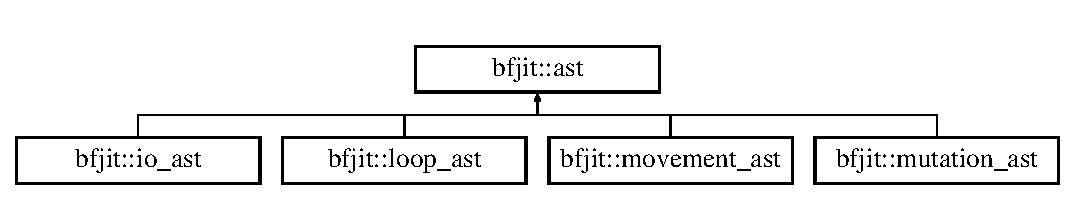
\includegraphics[height=2.000000cm]{classbfjit_1_1ast}
\end{center}
\end{figure}
\subsection*{Public Member Functions}
\begin{DoxyCompactItemize}
\item 
\hypertarget{classbfjit_1_1ast_a031935f8ba5af7185e8d75d67c1973dc}{}\label{classbfjit_1_1ast_a031935f8ba5af7185e8d75d67c1973dc} 
virtual \hyperlink{classbfjit_1_1ast_a031935f8ba5af7185e8d75d67c1973dc}{$\sim$ast} () noexcept=default
\begin{DoxyCompactList}\small\item\em Destroys the object. \end{DoxyCompactList}\item 
\hypertarget{classbfjit_1_1ast_a748b75683a33e11ad87b907ba0118c3d}{}\label{classbfjit_1_1ast_a748b75683a33e11ad87b907ba0118c3d} 
const \hyperlink{classbfjit_1_1position}{position} \& \hyperlink{classbfjit_1_1ast_a748b75683a33e11ad87b907ba0118c3d}{pos} () const noexcept
\begin{DoxyCompactList}\small\item\em Returns the position of this instruction in the stream. \end{DoxyCompactList}\end{DoxyCompactItemize}
\subsection*{Protected Member Functions}
\begin{DoxyCompactItemize}
\item 
\hypertarget{classbfjit_1_1ast_a6b8483df6623f32b184f6cf43fb6bcc1}{}\label{classbfjit_1_1ast_a6b8483df6623f32b184f6cf43fb6bcc1} 
\hyperlink{classbfjit_1_1ast_a6b8483df6623f32b184f6cf43fb6bcc1}{ast} (const \hyperlink{classbfjit_1_1position}{position} \&\hyperlink{classbfjit_1_1ast_a748b75683a33e11ad87b907ba0118c3d}{pos}) noexcept
\begin{DoxyCompactList}\small\item\em Constructs a new object, given its position. \end{DoxyCompactList}\item 
\hypertarget{classbfjit_1_1ast_aac08f2c318e8ccce75bd5028b48eaa91}{}\label{classbfjit_1_1ast_aac08f2c318e8ccce75bd5028b48eaa91} 
\hyperlink{classbfjit_1_1ast_aac08f2c318e8ccce75bd5028b48eaa91}{ast} (const \hyperlink{classbfjit_1_1ast}{ast} \&src) noexcept=default
\begin{DoxyCompactList}\small\item\em Constructs a new object, given an existing object. \end{DoxyCompactList}\item 
\hypertarget{classbfjit_1_1ast_a256a788db24653878f8e935945ddf0ed}{}\label{classbfjit_1_1ast_a256a788db24653878f8e935945ddf0ed} 
\hyperlink{classbfjit_1_1ast_a256a788db24653878f8e935945ddf0ed}{ast} (\hyperlink{classbfjit_1_1ast}{ast} \&\&src) noexcept=default
\begin{DoxyCompactList}\small\item\em Constructs a new object, given an existing temporary object. \end{DoxyCompactList}\end{DoxyCompactItemize}
\subsection*{Protected Attributes}
\begin{DoxyCompactItemize}
\item 
\hypertarget{classbfjit_1_1ast_a376d0d491063ec18be68d2e22b361d89}{}\label{classbfjit_1_1ast_a376d0d491063ec18be68d2e22b361d89} 
\hyperlink{classbfjit_1_1position}{position} \hyperlink{classbfjit_1_1ast_a376d0d491063ec18be68d2e22b361d89}{m\+\_\+pos}
\begin{DoxyCompactList}\small\item\em The position of ast in the stream. \end{DoxyCompactList}\end{DoxyCompactItemize}


\subsection{Detailed Description}
Abstract base class of all other ast classes. 

The documentation for this class was generated from the following files\+:\begin{DoxyCompactItemize}
\item 
include/ast.\+hpp\item 
src/ast.\+cpp\end{DoxyCompactItemize}

\hypertarget{classbfjit_1_1io__ast}{}\section{bfjit\+:\+:io\+\_\+ast Class Reference}
\label{classbfjit_1_1io__ast}\index{bfjit\+::io\+\_\+ast@{bfjit\+::io\+\_\+ast}}


A class that represent a single I/O instruction.  




{\ttfamily \#include $<$ast.\+hpp$>$}

Inheritance diagram for bfjit\+:\+:io\+\_\+ast\+:\begin{figure}[H]
\begin{center}
\leavevmode
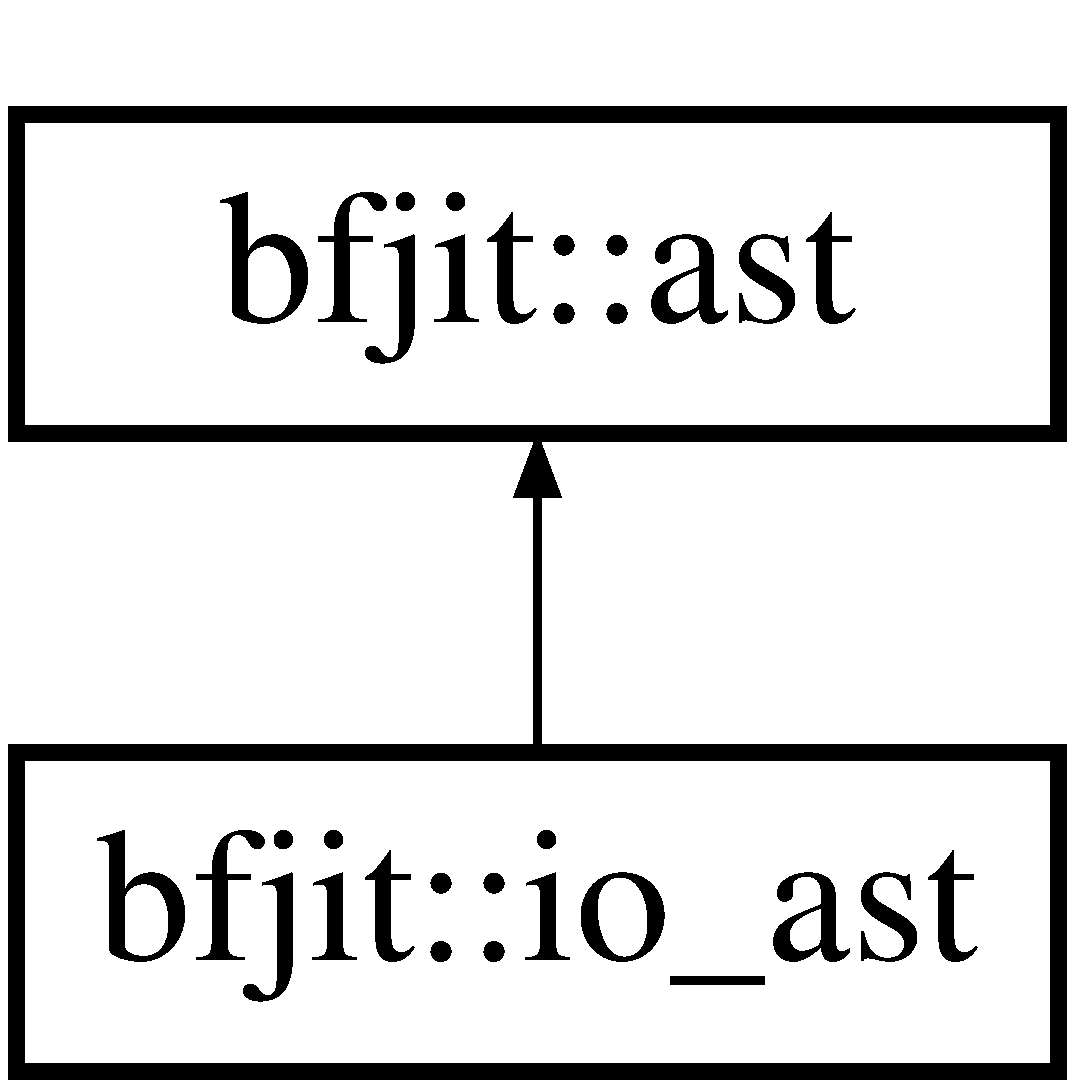
\includegraphics[height=2.000000cm]{classbfjit_1_1io__ast}
\end{center}
\end{figure}
\subsection*{Public Types}
\begin{DoxyCompactItemize}
\item 
enum \hyperlink{classbfjit_1_1io__ast_ae0b93ddde6f86aed45dd22b72d290414}{type} \+: std\+::uint\+\_\+fast8\+\_\+t \{ \hyperlink{classbfjit_1_1io__ast_ae0b93ddde6f86aed45dd22b72d290414ac86ee0d9d7ed3e7b4fdbf486fa6c0ebb}{type\+::\+IN}, 
\hyperlink{classbfjit_1_1io__ast_ae0b93ddde6f86aed45dd22b72d290414aef373774188a51f80463f37b6bd9e83a}{type\+::\+O\+UT}, 
\hyperlink{classbfjit_1_1io__ast_ae0b93ddde6f86aed45dd22b72d290414a62bd5a4afef994ba01e631cbf00f85be}{type\+::\+\_\+\+\_\+\+L\+A\+S\+T\+\_\+\+\_\+}
 \}\begin{DoxyCompactList}\small\item\em An enum that contains all possible types of I/O instructions. \end{DoxyCompactList}
\end{DoxyCompactItemize}
\subsection*{Public Member Functions}
\begin{DoxyCompactItemize}
\item 
\hypertarget{classbfjit_1_1io__ast_ae1806cd887145045a5adae13dd2febc9}{}\label{classbfjit_1_1io__ast_ae1806cd887145045a5adae13dd2febc9} 
\hyperlink{classbfjit_1_1io__ast_ae1806cd887145045a5adae13dd2febc9}{io\+\_\+ast} (const \hyperlink{classbfjit_1_1position}{position} \&\hyperlink{classbfjit_1_1ast_a748b75683a33e11ad87b907ba0118c3d}{pos}, const \hyperlink{classbfjit_1_1io__ast_ae0b93ddde6f86aed45dd22b72d290414}{type} \&\hyperlink{classbfjit_1_1io__ast_a9f8324f95fa4cb43d16fc8d44b5066ea}{ty}) noexcept
\begin{DoxyCompactList}\small\item\em Constructs a new object, given its position and type. \end{DoxyCompactList}\item 
\hypertarget{classbfjit_1_1io__ast_ac8bf6505bbeebba0cf423c434fa69714}{}\label{classbfjit_1_1io__ast_ac8bf6505bbeebba0cf423c434fa69714} 
\hyperlink{classbfjit_1_1io__ast_ac8bf6505bbeebba0cf423c434fa69714}{io\+\_\+ast} (const \hyperlink{classbfjit_1_1io__ast}{io\+\_\+ast} \&src) noexcept=default
\begin{DoxyCompactList}\small\item\em Constructs a new object, given an existing object. \end{DoxyCompactList}\item 
\hypertarget{classbfjit_1_1io__ast_aed38e58dc90bf5d01afe83b185ad3470}{}\label{classbfjit_1_1io__ast_aed38e58dc90bf5d01afe83b185ad3470} 
\hyperlink{classbfjit_1_1io__ast_aed38e58dc90bf5d01afe83b185ad3470}{io\+\_\+ast} (\hyperlink{classbfjit_1_1io__ast}{io\+\_\+ast} \&\&src) noexcept=default
\begin{DoxyCompactList}\small\item\em Constructs a new object, given an existing temporary object. \end{DoxyCompactList}\item 
\hypertarget{classbfjit_1_1io__ast_abcf50683af099523532e79fa124ebf8d}{}\label{classbfjit_1_1io__ast_abcf50683af099523532e79fa124ebf8d} 
\hyperlink{classbfjit_1_1io__ast_abcf50683af099523532e79fa124ebf8d}{$\sim$io\+\_\+ast} () noexcept override=default
\begin{DoxyCompactList}\small\item\em Destroys the object. \end{DoxyCompactList}\item 
\hypertarget{classbfjit_1_1io__ast_a9f8324f95fa4cb43d16fc8d44b5066ea}{}\label{classbfjit_1_1io__ast_a9f8324f95fa4cb43d16fc8d44b5066ea} 
const \hyperlink{classbfjit_1_1io__ast_ae0b93ddde6f86aed45dd22b72d290414}{type} \& \hyperlink{classbfjit_1_1io__ast_a9f8324f95fa4cb43d16fc8d44b5066ea}{ty} () const noexcept
\begin{DoxyCompactList}\small\item\em Returns the type of this I/O instruction. \end{DoxyCompactList}\end{DoxyCompactItemize}
\subsection*{Additional Inherited Members}


\subsection{Detailed Description}
A class that represent a single I/O instruction. 

Like other \hyperlink{namespacebfjit}{bfjit} classes, objects of this class are {\bfseries immutable}. 

\subsection{Member Enumeration Documentation}
\hypertarget{classbfjit_1_1io__ast_ae0b93ddde6f86aed45dd22b72d290414}{}\label{classbfjit_1_1io__ast_ae0b93ddde6f86aed45dd22b72d290414} 
\index{bfjit\+::io\+\_\+ast@{bfjit\+::io\+\_\+ast}!type@{type}}
\index{type@{type}!bfjit\+::io\+\_\+ast@{bfjit\+::io\+\_\+ast}}
\subsubsection{\texorpdfstring{type}{type}}
{\footnotesize\ttfamily enum \hyperlink{classbfjit_1_1io__ast_ae0b93ddde6f86aed45dd22b72d290414}{bfjit\+::io\+\_\+ast\+::type} \+: std\+::uint\+\_\+fast8\+\_\+t\hspace{0.3cm}{\ttfamily [strong]}}



An enum that contains all possible types of I/O instructions. 

\begin{DoxyEnumFields}{Enumerator}
\raisebox{\heightof{T}}[0pt][0pt]{\index{IN@{IN}!bfjit\+::io\+\_\+ast@{bfjit\+::io\+\_\+ast}}\index{bfjit\+::io\+\_\+ast@{bfjit\+::io\+\_\+ast}!IN@{IN}}}\hypertarget{classbfjit_1_1io__ast_ae0b93ddde6f86aed45dd22b72d290414ac86ee0d9d7ed3e7b4fdbf486fa6c0ebb}{}\label{classbfjit_1_1io__ast_ae0b93ddde6f86aed45dd22b72d290414ac86ee0d9d7ed3e7b4fdbf486fa6c0ebb} 
IN&Represents an {\itshape input number} instruction. \\
\hline

\raisebox{\heightof{T}}[0pt][0pt]{\index{O\+UT@{O\+UT}!bfjit\+::io\+\_\+ast@{bfjit\+::io\+\_\+ast}}\index{bfjit\+::io\+\_\+ast@{bfjit\+::io\+\_\+ast}!O\+UT@{O\+UT}}}\hypertarget{classbfjit_1_1io__ast_ae0b93ddde6f86aed45dd22b72d290414aef373774188a51f80463f37b6bd9e83a}{}\label{classbfjit_1_1io__ast_ae0b93ddde6f86aed45dd22b72d290414aef373774188a51f80463f37b6bd9e83a} 
O\+UT&Represents an {\itshape output number} instruction. \\
\hline

\raisebox{\heightof{T}}[0pt][0pt]{\index{\+\_\+\+\_\+\+L\+A\+S\+T\+\_\+\+\_\+@{\+\_\+\+\_\+\+L\+A\+S\+T\+\_\+\+\_\+}!bfjit\+::io\+\_\+ast@{bfjit\+::io\+\_\+ast}}\index{bfjit\+::io\+\_\+ast@{bfjit\+::io\+\_\+ast}!\+\_\+\+\_\+\+L\+A\+S\+T\+\_\+\+\_\+@{\+\_\+\+\_\+\+L\+A\+S\+T\+\_\+\+\_\+}}}\hypertarget{classbfjit_1_1io__ast_ae0b93ddde6f86aed45dd22b72d290414a62bd5a4afef994ba01e631cbf00f85be}{}\label{classbfjit_1_1io__ast_ae0b93ddde6f86aed45dd22b72d290414a62bd5a4afef994ba01e631cbf00f85be} 
\+\_\+\+\_\+\+L\+A\+S\+T\+\_\+\+\_\+&Number of enum entries. {\bfseries I\+N\+V\+A\+L\+ID V\+A\+L\+UE} \\
\hline

\end{DoxyEnumFields}


The documentation for this class was generated from the following files\+:\begin{DoxyCompactItemize}
\item 
include/ast.\+hpp\item 
src/ast.\+cpp\end{DoxyCompactItemize}

\hypertarget{classbfjit_1_1jit__function}{}\section{bfjit\+:\+:jit\+\_\+function Class Reference}
\label{classbfjit_1_1jit__function}\index{bfjit\+::jit\+\_\+function@{bfjit\+::jit\+\_\+function}}


A class that represents code ready for execution.  




{\ttfamily \#include $<$jit.\+hpp$>$}

\subsection*{Public Member Functions}
\begin{DoxyCompactItemize}
\item 
\hypertarget{classbfjit_1_1jit__function_af1fc2ce0a88008b14b83af58850ba986}{}\label{classbfjit_1_1jit__function_af1fc2ce0a88008b14b83af58850ba986} 
\hyperlink{classbfjit_1_1jit__function_af1fc2ce0a88008b14b83af58850ba986}{jit\+\_\+function} (const \hyperlink{classbfjit_1_1jit__function}{jit\+\_\+function} \&src)=delete
\begin{DoxyCompactList}\small\item\em \hyperlink{classbfjit_1_1jit__function}{jit\+\_\+function} cannot be copied. \end{DoxyCompactList}\item 
\hypertarget{classbfjit_1_1jit__function_a5d0022ddb357ff4671fd7b531a6a50c8}{}\label{classbfjit_1_1jit__function_a5d0022ddb357ff4671fd7b531a6a50c8} 
\hyperlink{classbfjit_1_1jit__function_a5d0022ddb357ff4671fd7b531a6a50c8}{jit\+\_\+function} (\hyperlink{classbfjit_1_1jit__function}{jit\+\_\+function} \&\&src)=default
\begin{DoxyCompactList}\small\item\em Constructs a new object, given an existing temporary object. \end{DoxyCompactList}\item 
\hypertarget{classbfjit_1_1jit__function_a01b04a52531720d33b15710f9439175b}{}\label{classbfjit_1_1jit__function_a01b04a52531720d33b15710f9439175b} 
\hyperlink{classbfjit_1_1jit__function_a01b04a52531720d33b15710f9439175b}{$\sim$jit\+\_\+function} ()
\begin{DoxyCompactList}\small\item\em Destroys the object. \end{DoxyCompactList}\item 
\hypertarget{classbfjit_1_1jit__function_a656a098b23685e1d27b9257b2981a046}{}\label{classbfjit_1_1jit__function_a656a098b23685e1d27b9257b2981a046} 
void \hyperlink{classbfjit_1_1jit__function_a656a098b23685e1d27b9257b2981a046}{operator()} () const
\begin{DoxyCompactList}\small\item\em Actually runs the generated code. \end{DoxyCompactList}\end{DoxyCompactItemize}
\subsection*{Static Public Member Functions}
\begin{DoxyCompactItemize}
\item 
static \hyperlink{classbfjit_1_1jit__function}{jit\+\_\+function} \hyperlink{classbfjit_1_1jit__function_a38edcf55a13c5766b8b832abcf19ac2b}{make} (std\+::vector$<$ \hyperlink{namespacebfjit_ad9bbdb76861e57928b1bc7695c2c0623}{combined\+\_\+ast} $>$\+::const\+\_\+iterator begin\+\_\+it, std\+::vector$<$ \hyperlink{namespacebfjit_ad9bbdb76861e57928b1bc7695c2c0623}{combined\+\_\+ast} $>$\+::const\+\_\+iterator end\+\_\+it, std\+::uint8\+\_\+t $\ast$bytes)
\begin{DoxyCompactList}\small\item\em {\itshape The} function for generating a \hyperlink{classbfjit_1_1jit__function}{jit\+\_\+function}. \end{DoxyCompactList}\end{DoxyCompactItemize}


\subsection{Detailed Description}
A class that represents code ready for execution. 

\subsection{Member Function Documentation}
\hypertarget{classbfjit_1_1jit__function_a38edcf55a13c5766b8b832abcf19ac2b}{}\label{classbfjit_1_1jit__function_a38edcf55a13c5766b8b832abcf19ac2b} 
\index{bfjit\+::jit\+\_\+function@{bfjit\+::jit\+\_\+function}!make@{make}}
\index{make@{make}!bfjit\+::jit\+\_\+function@{bfjit\+::jit\+\_\+function}}
\subsubsection{\texorpdfstring{make()}{make()}}
{\footnotesize\ttfamily static \hyperlink{classbfjit_1_1jit__function}{jit\+\_\+function} bfjit\+::jit\+\_\+function\+::make (\begin{DoxyParamCaption}\item[{std\+::vector$<$ \hyperlink{namespacebfjit_ad9bbdb76861e57928b1bc7695c2c0623}{combined\+\_\+ast} $>$\+::const\+\_\+iterator}]{begin\+\_\+it,  }\item[{std\+::vector$<$ \hyperlink{namespacebfjit_ad9bbdb76861e57928b1bc7695c2c0623}{combined\+\_\+ast} $>$\+::const\+\_\+iterator}]{end\+\_\+it,  }\item[{std\+::uint8\+\_\+t $\ast$}]{bytes }\end{DoxyParamCaption})\hspace{0.3cm}{\ttfamily [static]}}



{\itshape The} function for generating a \hyperlink{classbfjit_1_1jit__function}{jit\+\_\+function}. 


\begin{DoxyParams}{Parameters}
{\em begin\+\_\+it} & An iterator to the beginning of the code to jit. \\
\hline
{\em end\+\_\+it} & An iterator to the end of the code to jit. \\
\hline
{\em bytes} & Pointer to the cell heap. \\
\hline
\end{DoxyParams}


The documentation for this class was generated from the following file\+:\begin{DoxyCompactItemize}
\item 
include/jit.\+hpp\end{DoxyCompactItemize}

\hypertarget{classbfjit_1_1loop__ast}{}\section{bfjit\+:\+:loop\+\_\+ast Class Reference}
\label{classbfjit_1_1loop__ast}\index{bfjit\+::loop\+\_\+ast@{bfjit\+::loop\+\_\+ast}}


A class that represents a brainfuck loop.  




{\ttfamily \#include $<$ast.\+hpp$>$}

Inheritance diagram for bfjit\+:\+:loop\+\_\+ast\+:\begin{figure}[H]
\begin{center}
\leavevmode
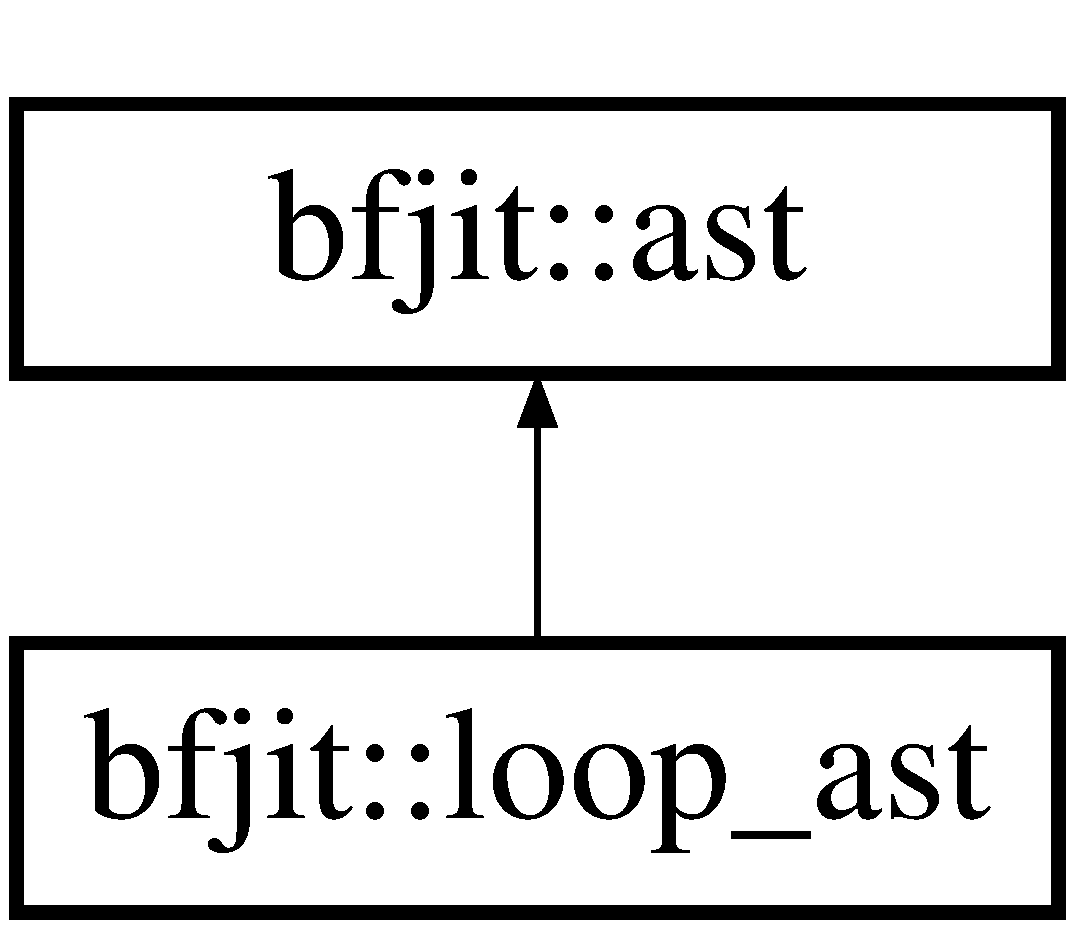
\includegraphics[height=2.000000cm]{classbfjit_1_1loop__ast}
\end{center}
\end{figure}
\subsection*{Public Member Functions}
\begin{DoxyCompactItemize}
\item 
\hypertarget{classbfjit_1_1loop__ast_ad30dcb55d7c06077ee2dafb1a378c5e7}{}\label{classbfjit_1_1loop__ast_ad30dcb55d7c06077ee2dafb1a378c5e7} 
\hyperlink{classbfjit_1_1loop__ast_ad30dcb55d7c06077ee2dafb1a378c5e7}{loop\+\_\+ast} (const \hyperlink{classbfjit_1_1position}{position} \&\hyperlink{classbfjit_1_1ast_a748b75683a33e11ad87b907ba0118c3d}{pos}, const std\+::vector$<$ \hyperlink{namespacebfjit_ad9bbdb76861e57928b1bc7695c2c0623}{combined\+\_\+ast} $>$ \&\hyperlink{classbfjit_1_1loop__ast_ad1418cddc65f555771317745baa12ca3}{inner})
\begin{DoxyCompactList}\small\item\em Constructs a new object, given its position and body. \end{DoxyCompactList}\item 
\hypertarget{classbfjit_1_1loop__ast_a755299be080720eb34d97cbd6f6d490f}{}\label{classbfjit_1_1loop__ast_a755299be080720eb34d97cbd6f6d490f} 
\hyperlink{classbfjit_1_1loop__ast_a755299be080720eb34d97cbd6f6d490f}{loop\+\_\+ast} (const \hyperlink{classbfjit_1_1loop__ast}{loop\+\_\+ast} \&src)=default
\begin{DoxyCompactList}\small\item\em Constructs a new object, given an existing object. \end{DoxyCompactList}\item 
\hypertarget{classbfjit_1_1loop__ast_a6d317229408e8ce7b77a779854228643}{}\label{classbfjit_1_1loop__ast_a6d317229408e8ce7b77a779854228643} 
\hyperlink{classbfjit_1_1loop__ast_a6d317229408e8ce7b77a779854228643}{loop\+\_\+ast} (\hyperlink{classbfjit_1_1loop__ast}{loop\+\_\+ast} \&\&src) noexcept=default
\begin{DoxyCompactList}\small\item\em Constructs a new object, given an existing temporary object. \end{DoxyCompactList}\item 
\hypertarget{classbfjit_1_1loop__ast_aae5b7064e86488f937b255307bd7d5d3}{}\label{classbfjit_1_1loop__ast_aae5b7064e86488f937b255307bd7d5d3} 
\hyperlink{classbfjit_1_1loop__ast_aae5b7064e86488f937b255307bd7d5d3}{$\sim$loop\+\_\+ast} () noexcept override=default
\begin{DoxyCompactList}\small\item\em Destroys the object. \end{DoxyCompactList}\item 
\hypertarget{classbfjit_1_1loop__ast_ad1418cddc65f555771317745baa12ca3}{}\label{classbfjit_1_1loop__ast_ad1418cddc65f555771317745baa12ca3} 
const std\+::vector$<$ \hyperlink{namespacebfjit_ad9bbdb76861e57928b1bc7695c2c0623}{combined\+\_\+ast} $>$ \& \hyperlink{classbfjit_1_1loop__ast_ad1418cddc65f555771317745baa12ca3}{inner} () const noexcept
\begin{DoxyCompactList}\small\item\em Returns the instructions containted within the loop. \end{DoxyCompactList}\end{DoxyCompactItemize}
\subsection*{Additional Inherited Members}


\subsection{Detailed Description}
A class that represents a brainfuck loop. 

Like other \hyperlink{namespacebfjit}{bfjit} classes, objects of this class are {\bfseries immutable}. 

The documentation for this class was generated from the following files\+:\begin{DoxyCompactItemize}
\item 
include/ast.\+hpp\item 
src/ast.\+cpp\end{DoxyCompactItemize}

\hypertarget{classbfjit_1_1movement__ast}{}\section{bfjit\+:\+:movement\+\_\+ast Class Reference}
\label{classbfjit_1_1movement__ast}\index{bfjit\+::movement\+\_\+ast@{bfjit\+::movement\+\_\+ast}}


A class that represents a movement instruction.  




{\ttfamily \#include $<$ast.\+hpp$>$}

Inheritance diagram for bfjit\+:\+:movement\+\_\+ast\+:\begin{figure}[H]
\begin{center}
\leavevmode
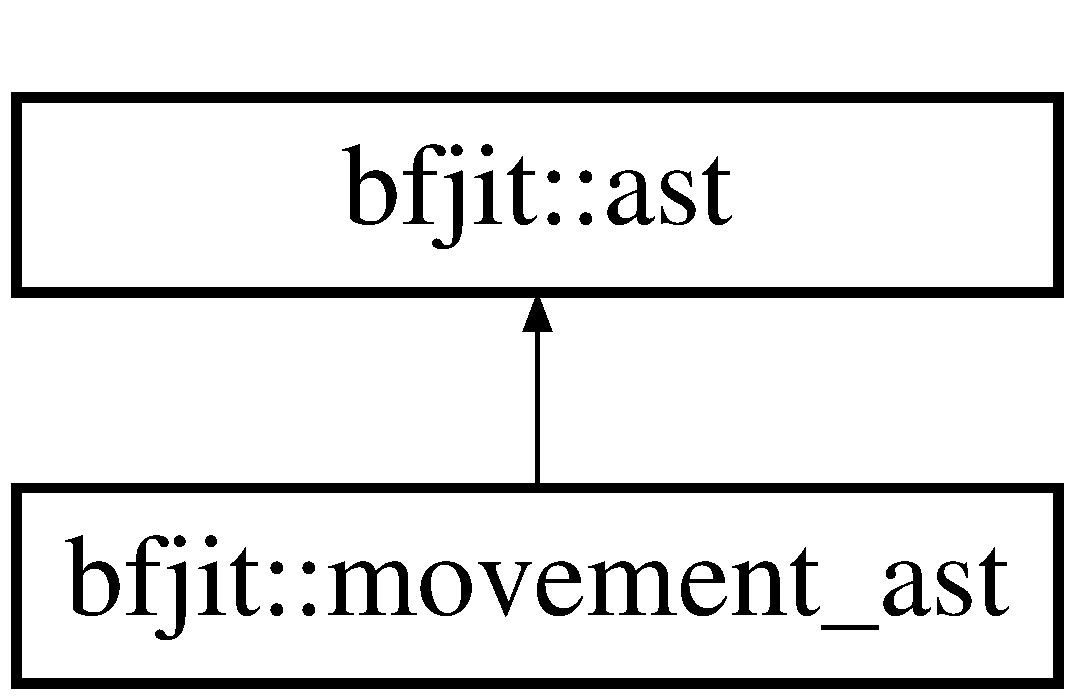
\includegraphics[height=2.000000cm]{classbfjit_1_1movement__ast}
\end{center}
\end{figure}
\subsection*{Public Types}
\begin{DoxyCompactItemize}
\item 
enum \hyperlink{classbfjit_1_1movement__ast_a3aa723a03d76c31e1e88be817670701f}{type} \+: std\+::uint\+\_\+fast8\+\_\+t \{ \hyperlink{classbfjit_1_1movement__ast_a3aa723a03d76c31e1e88be817670701fa684d325a7303f52e64011467ff5c5758}{type\+::\+L\+E\+FT}, 
\hyperlink{classbfjit_1_1movement__ast_a3aa723a03d76c31e1e88be817670701fa21507b40c80068eda19865706fdc2403}{type\+::\+R\+I\+G\+HT}, 
\hyperlink{classbfjit_1_1movement__ast_a3aa723a03d76c31e1e88be817670701fa62bd5a4afef994ba01e631cbf00f85be}{type\+::\+\_\+\+\_\+\+L\+A\+S\+T\+\_\+\+\_\+}
 \}\begin{DoxyCompactList}\small\item\em An enum that contains all possible types of movement instructions. \end{DoxyCompactList}
\end{DoxyCompactItemize}
\subsection*{Public Member Functions}
\begin{DoxyCompactItemize}
\item 
\hypertarget{classbfjit_1_1movement__ast_a3e0eae96553010515592ab54a983517b}{}\label{classbfjit_1_1movement__ast_a3e0eae96553010515592ab54a983517b} 
\hyperlink{classbfjit_1_1movement__ast_a3e0eae96553010515592ab54a983517b}{movement\+\_\+ast} (const \hyperlink{classbfjit_1_1position}{position} \&\hyperlink{classbfjit_1_1ast_a748b75683a33e11ad87b907ba0118c3d}{pos}, const \hyperlink{classbfjit_1_1movement__ast_a3aa723a03d76c31e1e88be817670701f}{type} \&\hyperlink{classbfjit_1_1movement__ast_ad96cbdcde5bb9ea928896fe8fccf7eae}{ty}, const size\+\_\+t \&\hyperlink{classbfjit_1_1movement__ast_ad8d951b3fb908d5f4316214d95162462}{by}) noexcept
\begin{DoxyCompactList}\small\item\em Constructs a new object, given its position, type and the number of moves to perform. \end{DoxyCompactList}\item 
\hypertarget{classbfjit_1_1movement__ast_a49f3fad998b07d9cba3daa1cab5e4e7e}{}\label{classbfjit_1_1movement__ast_a49f3fad998b07d9cba3daa1cab5e4e7e} 
\hyperlink{classbfjit_1_1movement__ast_a49f3fad998b07d9cba3daa1cab5e4e7e}{movement\+\_\+ast} (const \hyperlink{classbfjit_1_1movement__ast}{movement\+\_\+ast} \&src) noexcept=default
\begin{DoxyCompactList}\small\item\em Constructs a new object, given an existing object. \end{DoxyCompactList}\item 
\hypertarget{classbfjit_1_1movement__ast_af588abab4c5b0e5fca3c4a94260ac7b2}{}\label{classbfjit_1_1movement__ast_af588abab4c5b0e5fca3c4a94260ac7b2} 
\hyperlink{classbfjit_1_1movement__ast_af588abab4c5b0e5fca3c4a94260ac7b2}{movement\+\_\+ast} (\hyperlink{classbfjit_1_1movement__ast}{movement\+\_\+ast} \&\&src) noexcept=default
\begin{DoxyCompactList}\small\item\em Constructs a new object, given an existing temporary object. \end{DoxyCompactList}\item 
\hypertarget{classbfjit_1_1movement__ast_a145ac93e5fa7fc7bcbfddc6d6d4c0d83}{}\label{classbfjit_1_1movement__ast_a145ac93e5fa7fc7bcbfddc6d6d4c0d83} 
\hyperlink{classbfjit_1_1movement__ast_a145ac93e5fa7fc7bcbfddc6d6d4c0d83}{$\sim$movement\+\_\+ast} () noexcept override=default
\begin{DoxyCompactList}\small\item\em Destroys the object. \end{DoxyCompactList}\item 
\hypertarget{classbfjit_1_1movement__ast_ad96cbdcde5bb9ea928896fe8fccf7eae}{}\label{classbfjit_1_1movement__ast_ad96cbdcde5bb9ea928896fe8fccf7eae} 
const \hyperlink{classbfjit_1_1movement__ast_a3aa723a03d76c31e1e88be817670701f}{type} \& \hyperlink{classbfjit_1_1movement__ast_ad96cbdcde5bb9ea928896fe8fccf7eae}{ty} () const noexcept
\begin{DoxyCompactList}\small\item\em Returns the type of this movement instruction. \end{DoxyCompactList}\item 
\hypertarget{classbfjit_1_1movement__ast_ad8d951b3fb908d5f4316214d95162462}{}\label{classbfjit_1_1movement__ast_ad8d951b3fb908d5f4316214d95162462} 
const size\+\_\+t \& \hyperlink{classbfjit_1_1movement__ast_ad8d951b3fb908d5f4316214d95162462}{by} () const noexcept
\begin{DoxyCompactList}\small\item\em Returns the amount which the pointer needs to move {\itshape by}. \end{DoxyCompactList}\end{DoxyCompactItemize}
\subsection*{Additional Inherited Members}


\subsection{Detailed Description}
A class that represents a movement instruction. 

Like other \hyperlink{namespacebfjit}{bfjit} classes, objects of this class are {\bfseries immutable}. 

\subsection{Member Enumeration Documentation}
\hypertarget{classbfjit_1_1movement__ast_a3aa723a03d76c31e1e88be817670701f}{}\label{classbfjit_1_1movement__ast_a3aa723a03d76c31e1e88be817670701f} 
\index{bfjit\+::movement\+\_\+ast@{bfjit\+::movement\+\_\+ast}!type@{type}}
\index{type@{type}!bfjit\+::movement\+\_\+ast@{bfjit\+::movement\+\_\+ast}}
\subsubsection{\texorpdfstring{type}{type}}
{\footnotesize\ttfamily enum \hyperlink{classbfjit_1_1movement__ast_a3aa723a03d76c31e1e88be817670701f}{bfjit\+::movement\+\_\+ast\+::type} \+: std\+::uint\+\_\+fast8\+\_\+t\hspace{0.3cm}{\ttfamily [strong]}}



An enum that contains all possible types of movement instructions. 

\begin{DoxyEnumFields}{Enumerator}
\raisebox{\heightof{T}}[0pt][0pt]{\index{L\+E\+FT@{L\+E\+FT}!bfjit\+::movement\+\_\+ast@{bfjit\+::movement\+\_\+ast}}\index{bfjit\+::movement\+\_\+ast@{bfjit\+::movement\+\_\+ast}!L\+E\+FT@{L\+E\+FT}}}\hypertarget{classbfjit_1_1movement__ast_a3aa723a03d76c31e1e88be817670701fa684d325a7303f52e64011467ff5c5758}{}\label{classbfjit_1_1movement__ast_a3aa723a03d76c31e1e88be817670701fa684d325a7303f52e64011467ff5c5758} 
L\+E\+FT&Represents a {\itshape go left} instruction. \\
\hline

\raisebox{\heightof{T}}[0pt][0pt]{\index{R\+I\+G\+HT@{R\+I\+G\+HT}!bfjit\+::movement\+\_\+ast@{bfjit\+::movement\+\_\+ast}}\index{bfjit\+::movement\+\_\+ast@{bfjit\+::movement\+\_\+ast}!R\+I\+G\+HT@{R\+I\+G\+HT}}}\hypertarget{classbfjit_1_1movement__ast_a3aa723a03d76c31e1e88be817670701fa21507b40c80068eda19865706fdc2403}{}\label{classbfjit_1_1movement__ast_a3aa723a03d76c31e1e88be817670701fa21507b40c80068eda19865706fdc2403} 
R\+I\+G\+HT&Represents a {\itshape go right} instruction. \\
\hline

\raisebox{\heightof{T}}[0pt][0pt]{\index{\+\_\+\+\_\+\+L\+A\+S\+T\+\_\+\+\_\+@{\+\_\+\+\_\+\+L\+A\+S\+T\+\_\+\+\_\+}!bfjit\+::movement\+\_\+ast@{bfjit\+::movement\+\_\+ast}}\index{bfjit\+::movement\+\_\+ast@{bfjit\+::movement\+\_\+ast}!\+\_\+\+\_\+\+L\+A\+S\+T\+\_\+\+\_\+@{\+\_\+\+\_\+\+L\+A\+S\+T\+\_\+\+\_\+}}}\hypertarget{classbfjit_1_1movement__ast_a3aa723a03d76c31e1e88be817670701fa62bd5a4afef994ba01e631cbf00f85be}{}\label{classbfjit_1_1movement__ast_a3aa723a03d76c31e1e88be817670701fa62bd5a4afef994ba01e631cbf00f85be} 
\+\_\+\+\_\+\+L\+A\+S\+T\+\_\+\+\_\+&Number of enum entries. {\bfseries I\+N\+V\+A\+L\+ID V\+A\+L\+UE} \\
\hline

\end{DoxyEnumFields}


The documentation for this class was generated from the following files\+:\begin{DoxyCompactItemize}
\item 
include/ast.\+hpp\item 
src/ast.\+cpp\end{DoxyCompactItemize}

\hypertarget{classbfjit_1_1mutation__ast}{}\section{bfjit\+:\+:mutation\+\_\+ast Class Reference}
\label{classbfjit_1_1mutation__ast}\index{bfjit\+::mutation\+\_\+ast@{bfjit\+::mutation\+\_\+ast}}


A class that represents a single (cellmutation) instruction.  




{\ttfamily \#include $<$ast.\+hpp$>$}

Inheritance diagram for bfjit\+:\+:mutation\+\_\+ast\+:\begin{figure}[H]
\begin{center}
\leavevmode
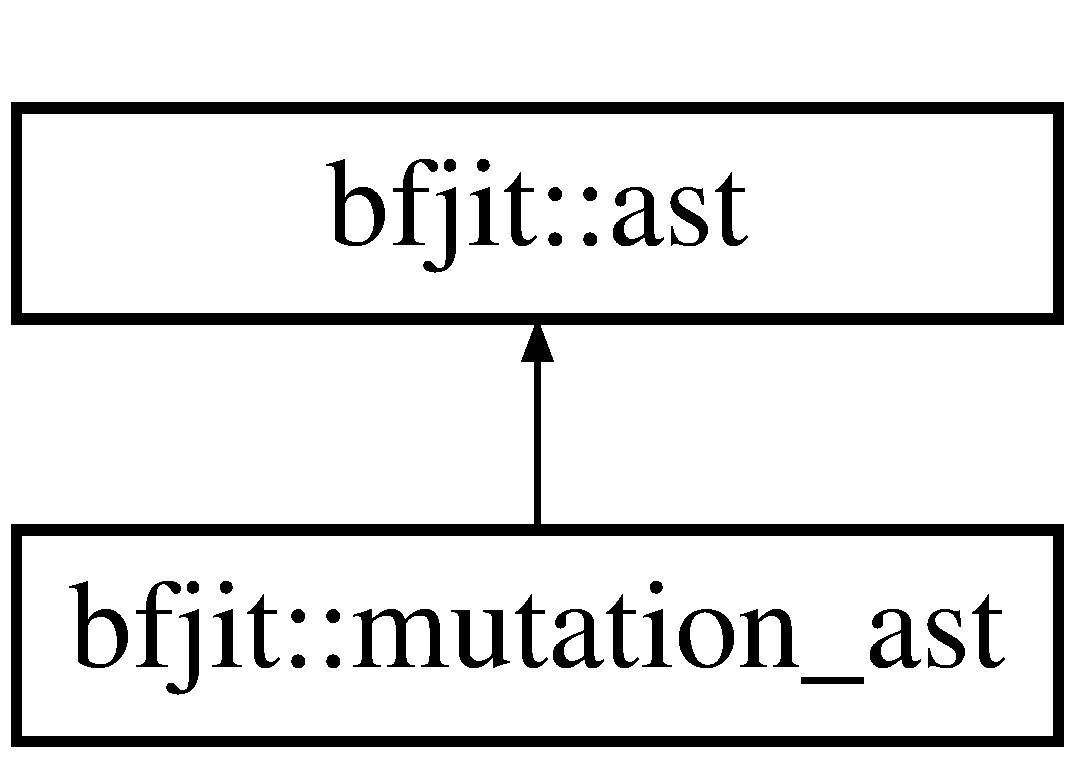
\includegraphics[height=2.000000cm]{classbfjit_1_1mutation__ast}
\end{center}
\end{figure}
\subsection*{Public Types}
\begin{DoxyCompactItemize}
\item 
enum \hyperlink{classbfjit_1_1mutation__ast_a4a35ab616dab7944deedac4300f473e9}{type} \+: std\+::uint\+\_\+fast8\+\_\+t \{ \hyperlink{classbfjit_1_1mutation__ast_a4a35ab616dab7944deedac4300f473e9a38924f2227ebf15f4bdc6dca5c5eca91}{type\+::\+I\+NC}, 
\hyperlink{classbfjit_1_1mutation__ast_a4a35ab616dab7944deedac4300f473e9a38344a4d87bb35ec197f26fad338b6ab}{type\+::\+D\+EC}, 
\hyperlink{classbfjit_1_1mutation__ast_a4a35ab616dab7944deedac4300f473e9a62bd5a4afef994ba01e631cbf00f85be}{type\+::\+\_\+\+\_\+\+L\+A\+S\+T\+\_\+\+\_\+}
 \}\begin{DoxyCompactList}\small\item\em An enum that contains all possible types of mutation instructions. \end{DoxyCompactList}
\end{DoxyCompactItemize}
\subsection*{Public Member Functions}
\begin{DoxyCompactItemize}
\item 
\hypertarget{classbfjit_1_1mutation__ast_aa4c4051e73b3e286a7587264de13c6fb}{}\label{classbfjit_1_1mutation__ast_aa4c4051e73b3e286a7587264de13c6fb} 
\hyperlink{classbfjit_1_1mutation__ast_aa4c4051e73b3e286a7587264de13c6fb}{mutation\+\_\+ast} (const \hyperlink{classbfjit_1_1position}{position} \&\hyperlink{classbfjit_1_1ast_a748b75683a33e11ad87b907ba0118c3d}{pos}, const \hyperlink{classbfjit_1_1mutation__ast_a4a35ab616dab7944deedac4300f473e9}{type} \&\hyperlink{classbfjit_1_1mutation__ast_a8f80ac1d17d4c77c1e5032f970e15e8e}{ty}, const size\+\_\+t \&\hyperlink{classbfjit_1_1mutation__ast_a2ee0d76e3a8aabee083952aea21035a5}{by}) noexcept
\begin{DoxyCompactList}\small\item\em Constructs a new object, given its position, type and the number of mutations to perform. \end{DoxyCompactList}\item 
\hypertarget{classbfjit_1_1mutation__ast_a13a88c3bab4ad64b00c5f00cb553a4df}{}\label{classbfjit_1_1mutation__ast_a13a88c3bab4ad64b00c5f00cb553a4df} 
\hyperlink{classbfjit_1_1mutation__ast_a13a88c3bab4ad64b00c5f00cb553a4df}{mutation\+\_\+ast} (const \hyperlink{classbfjit_1_1mutation__ast}{mutation\+\_\+ast} \&src) noexcept=default
\begin{DoxyCompactList}\small\item\em Constructs a new object, given an existing object. \end{DoxyCompactList}\item 
\hypertarget{classbfjit_1_1mutation__ast_a79a438bf768cea7e786ff38c971dd9aa}{}\label{classbfjit_1_1mutation__ast_a79a438bf768cea7e786ff38c971dd9aa} 
\hyperlink{classbfjit_1_1mutation__ast_a79a438bf768cea7e786ff38c971dd9aa}{mutation\+\_\+ast} (\hyperlink{classbfjit_1_1mutation__ast}{mutation\+\_\+ast} \&\&src) noexcept=default
\begin{DoxyCompactList}\small\item\em Constructs a new object, given an existing temporary object. \end{DoxyCompactList}\item 
\hypertarget{classbfjit_1_1mutation__ast_ae92ede7339103c1552ce76a4578c6bf7}{}\label{classbfjit_1_1mutation__ast_ae92ede7339103c1552ce76a4578c6bf7} 
\hyperlink{classbfjit_1_1mutation__ast_ae92ede7339103c1552ce76a4578c6bf7}{$\sim$mutation\+\_\+ast} () noexcept override=default
\begin{DoxyCompactList}\small\item\em Destroys the object. \end{DoxyCompactList}\item 
\hypertarget{classbfjit_1_1mutation__ast_a8f80ac1d17d4c77c1e5032f970e15e8e}{}\label{classbfjit_1_1mutation__ast_a8f80ac1d17d4c77c1e5032f970e15e8e} 
const \hyperlink{classbfjit_1_1mutation__ast_a4a35ab616dab7944deedac4300f473e9}{type} \& \hyperlink{classbfjit_1_1mutation__ast_a8f80ac1d17d4c77c1e5032f970e15e8e}{ty} () const noexcept
\begin{DoxyCompactList}\small\item\em Returns the type of this mutation instruction. \end{DoxyCompactList}\item 
\hypertarget{classbfjit_1_1mutation__ast_a2ee0d76e3a8aabee083952aea21035a5}{}\label{classbfjit_1_1mutation__ast_a2ee0d76e3a8aabee083952aea21035a5} 
const size\+\_\+t \& \hyperlink{classbfjit_1_1mutation__ast_a2ee0d76e3a8aabee083952aea21035a5}{by} () const noexcept
\begin{DoxyCompactList}\small\item\em Returns the amount which the cell needs to change {\itshape by}. \end{DoxyCompactList}\end{DoxyCompactItemize}
\subsection*{Additional Inherited Members}


\subsection{Detailed Description}
A class that represents a single (cellmutation) instruction. 

Like other \hyperlink{namespacebfjit}{bfjit} classes, objects of this class are {\bfseries immutable}. 

\subsection{Member Enumeration Documentation}
\hypertarget{classbfjit_1_1mutation__ast_a4a35ab616dab7944deedac4300f473e9}{}\label{classbfjit_1_1mutation__ast_a4a35ab616dab7944deedac4300f473e9} 
\index{bfjit\+::mutation\+\_\+ast@{bfjit\+::mutation\+\_\+ast}!type@{type}}
\index{type@{type}!bfjit\+::mutation\+\_\+ast@{bfjit\+::mutation\+\_\+ast}}
\subsubsection{\texorpdfstring{type}{type}}
{\footnotesize\ttfamily enum \hyperlink{classbfjit_1_1mutation__ast_a4a35ab616dab7944deedac4300f473e9}{bfjit\+::mutation\+\_\+ast\+::type} \+: std\+::uint\+\_\+fast8\+\_\+t\hspace{0.3cm}{\ttfamily [strong]}}



An enum that contains all possible types of mutation instructions. 

\begin{DoxyEnumFields}{Enumerator}
\raisebox{\heightof{T}}[0pt][0pt]{\index{I\+NC@{I\+NC}!bfjit\+::mutation\+\_\+ast@{bfjit\+::mutation\+\_\+ast}}\index{bfjit\+::mutation\+\_\+ast@{bfjit\+::mutation\+\_\+ast}!I\+NC@{I\+NC}}}\hypertarget{classbfjit_1_1mutation__ast_a4a35ab616dab7944deedac4300f473e9a38924f2227ebf15f4bdc6dca5c5eca91}{}\label{classbfjit_1_1mutation__ast_a4a35ab616dab7944deedac4300f473e9a38924f2227ebf15f4bdc6dca5c5eca91} 
I\+NC&Represents a {\itshape increase value} instruction. \\
\hline

\raisebox{\heightof{T}}[0pt][0pt]{\index{D\+EC@{D\+EC}!bfjit\+::mutation\+\_\+ast@{bfjit\+::mutation\+\_\+ast}}\index{bfjit\+::mutation\+\_\+ast@{bfjit\+::mutation\+\_\+ast}!D\+EC@{D\+EC}}}\hypertarget{classbfjit_1_1mutation__ast_a4a35ab616dab7944deedac4300f473e9a38344a4d87bb35ec197f26fad338b6ab}{}\label{classbfjit_1_1mutation__ast_a4a35ab616dab7944deedac4300f473e9a38344a4d87bb35ec197f26fad338b6ab} 
D\+EC&Represents a {\itshape decrease value} instruction. \\
\hline

\raisebox{\heightof{T}}[0pt][0pt]{\index{\+\_\+\+\_\+\+L\+A\+S\+T\+\_\+\+\_\+@{\+\_\+\+\_\+\+L\+A\+S\+T\+\_\+\+\_\+}!bfjit\+::mutation\+\_\+ast@{bfjit\+::mutation\+\_\+ast}}\index{bfjit\+::mutation\+\_\+ast@{bfjit\+::mutation\+\_\+ast}!\+\_\+\+\_\+\+L\+A\+S\+T\+\_\+\+\_\+@{\+\_\+\+\_\+\+L\+A\+S\+T\+\_\+\+\_\+}}}\hypertarget{classbfjit_1_1mutation__ast_a4a35ab616dab7944deedac4300f473e9a62bd5a4afef994ba01e631cbf00f85be}{}\label{classbfjit_1_1mutation__ast_a4a35ab616dab7944deedac4300f473e9a62bd5a4afef994ba01e631cbf00f85be} 
\+\_\+\+\_\+\+L\+A\+S\+T\+\_\+\+\_\+&Number of enum entries. {\bfseries I\+N\+V\+A\+L\+ID V\+A\+L\+UE} \\
\hline

\end{DoxyEnumFields}


The documentation for this class was generated from the following files\+:\begin{DoxyCompactItemize}
\item 
include/ast.\+hpp\item 
src/ast.\+cpp\end{DoxyCompactItemize}

\hypertarget{structoptions}{}\section{options Struct Reference}
\label{structoptions}\index{options@{options}}
\subsection*{Public Attributes}
\begin{DoxyCompactItemize}
\item 
\hypertarget{structoptions_a8af1b7603b6393be8711439e5c9985a4}{}\label{structoptions_a8af1b7603b6393be8711439e5c9985a4} 
bool \hyperlink{structoptions_a8af1b7603b6393be8711439e5c9985a4}{optimize}
\begin{DoxyCompactList}\small\item\em Specifies whether to optimize the generated ast. \end{DoxyCompactList}\item 
\hypertarget{structoptions_a70b2278d5fd6477af7fecf7e69a0e07b}{}\label{structoptions_a70b2278d5fd6477af7fecf7e69a0e07b} 
std\+::size\+\_\+t \hyperlink{structoptions_a70b2278d5fd6477af7fecf7e69a0e07b}{size}
\begin{DoxyCompactList}\small\item\em Specifies the size of the heap. \end{DoxyCompactList}\item 
\hypertarget{structoptions_a021db9b61479499c1d65da5dfa04b177}{}\label{structoptions_a021db9b61479499c1d65da5dfa04b177} 
std\+::string \hyperlink{structoptions_a021db9b61479499c1d65da5dfa04b177}{file\+\_\+name}
\begin{DoxyCompactList}\small\item\em Specifies the name of the input file. \end{DoxyCompactList}\item 
\hypertarget{structoptions_a8aafbc7ce4badfbaa8e2caf801b84a8e}{}\label{structoptions_a8aafbc7ce4badfbaa8e2caf801b84a8e} 
bool \hyperlink{structoptions_a8aafbc7ce4badfbaa8e2caf801b84a8e}{pbrain}
\begin{DoxyCompactList}\small\item\em Specifies whether to enable pbrain extension. \end{DoxyCompactList}\end{DoxyCompactItemize}


The documentation for this struct was generated from the following file\+:\begin{DoxyCompactItemize}
\item 
app/include/options.\+hpp\end{DoxyCompactItemize}

\hypertarget{classbfjit_1_1parse__error}{}\section{bfjit\+:\+:parse\+\_\+error Class Reference}
\label{classbfjit_1_1parse__error}\index{bfjit\+::parse\+\_\+error@{bfjit\+::parse\+\_\+error}}
\subsection*{Public Types}
\begin{DoxyCompactItemize}
\item 
enum \hyperlink{classbfjit_1_1parse__error_af750138d196890dcdc543c9fb1b7705b}{type} \+: std\+::uint\+\_\+fast8\+\_\+t \{ \hyperlink{classbfjit_1_1parse__error_af750138d196890dcdc543c9fb1b7705badb8aa960a3f467cff16772c10e9a4c07}{type\+::\+M\+I\+S\+M\+A\+T\+C\+H\+E\+D\+\_\+\+B\+R\+A\+C\+K\+E\+TS}, 
\hyperlink{classbfjit_1_1parse__error_af750138d196890dcdc543c9fb1b7705ba62bd5a4afef994ba01e631cbf00f85be}{type\+::\+\_\+\+\_\+\+L\+A\+S\+T\+\_\+\+\_\+}
 \}\begin{DoxyCompactList}\small\item\em An enum that contains all possible reasons that parsing can fail. \end{DoxyCompactList}
\end{DoxyCompactItemize}
\subsection*{Public Member Functions}
\begin{DoxyCompactItemize}
\item 
\hypertarget{classbfjit_1_1parse__error_a492dc45a5a66316cb51fb2b4259f674d}{}\label{classbfjit_1_1parse__error_a492dc45a5a66316cb51fb2b4259f674d} 
\hyperlink{classbfjit_1_1parse__error_a492dc45a5a66316cb51fb2b4259f674d}{parse\+\_\+error} (const \hyperlink{classbfjit_1_1parse__error_af750138d196890dcdc543c9fb1b7705b}{type} \&\hyperlink{classbfjit_1_1parse__error_ae4d7328b778c35873aefd3c76b85e38b}{ty}, const \hyperlink{classbfjit_1_1position}{position} \&\hyperlink{classbfjit_1_1parse__error_a5dd50c33cba31daa171f2809231c2fd2}{pos})
\begin{DoxyCompactList}\small\item\em Constructs a new object, given its type and position. \end{DoxyCompactList}\item 
\hypertarget{classbfjit_1_1parse__error_ae4d7328b778c35873aefd3c76b85e38b}{}\label{classbfjit_1_1parse__error_ae4d7328b778c35873aefd3c76b85e38b} 
const \hyperlink{classbfjit_1_1parse__error_af750138d196890dcdc543c9fb1b7705b}{type} \& \hyperlink{classbfjit_1_1parse__error_ae4d7328b778c35873aefd3c76b85e38b}{ty} () const
\begin{DoxyCompactList}\small\item\em Returns the type of this error. \end{DoxyCompactList}\item 
\hypertarget{classbfjit_1_1parse__error_a5dd50c33cba31daa171f2809231c2fd2}{}\label{classbfjit_1_1parse__error_a5dd50c33cba31daa171f2809231c2fd2} 
const \hyperlink{classbfjit_1_1position}{position} \& \hyperlink{classbfjit_1_1parse__error_a5dd50c33cba31daa171f2809231c2fd2}{pos} () const
\begin{DoxyCompactList}\small\item\em Returns the position of this error. \end{DoxyCompactList}\end{DoxyCompactItemize}


\subsection{Member Enumeration Documentation}
\hypertarget{classbfjit_1_1parse__error_af750138d196890dcdc543c9fb1b7705b}{}\label{classbfjit_1_1parse__error_af750138d196890dcdc543c9fb1b7705b} 
\index{bfjit\+::parse\+\_\+error@{bfjit\+::parse\+\_\+error}!type@{type}}
\index{type@{type}!bfjit\+::parse\+\_\+error@{bfjit\+::parse\+\_\+error}}
\subsubsection{\texorpdfstring{type}{type}}
{\footnotesize\ttfamily enum \hyperlink{classbfjit_1_1parse__error_af750138d196890dcdc543c9fb1b7705b}{bfjit\+::parse\+\_\+error\+::type} \+: std\+::uint\+\_\+fast8\+\_\+t\hspace{0.3cm}{\ttfamily [strong]}}



An enum that contains all possible reasons that parsing can fail. 

\begin{DoxyEnumFields}{Enumerator}
\raisebox{\heightof{T}}[0pt][0pt]{\index{M\+I\+S\+M\+A\+T\+C\+H\+E\+D\+\_\+\+B\+R\+A\+C\+K\+E\+TS@{M\+I\+S\+M\+A\+T\+C\+H\+E\+D\+\_\+\+B\+R\+A\+C\+K\+E\+TS}!bfjit\+::parse\+\_\+error@{bfjit\+::parse\+\_\+error}}\index{bfjit\+::parse\+\_\+error@{bfjit\+::parse\+\_\+error}!M\+I\+S\+M\+A\+T\+C\+H\+E\+D\+\_\+\+B\+R\+A\+C\+K\+E\+TS@{M\+I\+S\+M\+A\+T\+C\+H\+E\+D\+\_\+\+B\+R\+A\+C\+K\+E\+TS}}}\hypertarget{classbfjit_1_1parse__error_af750138d196890dcdc543c9fb1b7705badb8aa960a3f467cff16772c10e9a4c07}{}\label{classbfjit_1_1parse__error_af750138d196890dcdc543c9fb1b7705badb8aa960a3f467cff16772c10e9a4c07} 
M\+I\+S\+M\+A\+T\+C\+H\+E\+D\+\_\+\+B\+R\+A\+C\+K\+E\+TS&Indicates that brackets where mismatched. \\
\hline

\raisebox{\heightof{T}}[0pt][0pt]{\index{\+\_\+\+\_\+\+L\+A\+S\+T\+\_\+\+\_\+@{\+\_\+\+\_\+\+L\+A\+S\+T\+\_\+\+\_\+}!bfjit\+::parse\+\_\+error@{bfjit\+::parse\+\_\+error}}\index{bfjit\+::parse\+\_\+error@{bfjit\+::parse\+\_\+error}!\+\_\+\+\_\+\+L\+A\+S\+T\+\_\+\+\_\+@{\+\_\+\+\_\+\+L\+A\+S\+T\+\_\+\+\_\+}}}\hypertarget{classbfjit_1_1parse__error_af750138d196890dcdc543c9fb1b7705ba62bd5a4afef994ba01e631cbf00f85be}{}\label{classbfjit_1_1parse__error_af750138d196890dcdc543c9fb1b7705ba62bd5a4afef994ba01e631cbf00f85be} 
\+\_\+\+\_\+\+L\+A\+S\+T\+\_\+\+\_\+&Number of enum entries. {\bfseries I\+N\+V\+A\+L\+ID V\+A\+L\+UE} \\
\hline

\end{DoxyEnumFields}


The documentation for this class was generated from the following files\+:\begin{DoxyCompactItemize}
\item 
include/parse.\+hpp\item 
src/parse.\+cpp\end{DoxyCompactItemize}

\hypertarget{classbfjit_1_1position}{}\section{bfjit\+:\+:position Class Reference}
\label{classbfjit_1_1position}\index{bfjit\+::position@{bfjit\+::position}}


A class that tracks position of a token in a stream.  




{\ttfamily \#include $<$position.\+hpp$>$}

\subsection*{Public Types}
\begin{DoxyCompactItemize}
\item 
\hypertarget{classbfjit_1_1position_a6319989e5821e4a159ed1870e8ba656e}{}\label{classbfjit_1_1position_a6319989e5821e4a159ed1870e8ba656e} 
using \hyperlink{classbfjit_1_1position_a6319989e5821e4a159ed1870e8ba656e}{line\+\_\+type} = std\+::uint\+\_\+fast32\+\_\+t
\begin{DoxyCompactList}\small\item\em A simple typedef for line numbers. \end{DoxyCompactList}\item 
\hypertarget{classbfjit_1_1position_a472af3de5d41775deff6293c0ab6450b}{}\label{classbfjit_1_1position_a472af3de5d41775deff6293c0ab6450b} 
using \hyperlink{classbfjit_1_1position_a472af3de5d41775deff6293c0ab6450b}{column\+\_\+type} = std\+::uint\+\_\+fast32\+\_\+t
\begin{DoxyCompactList}\small\item\em A simple typedef for column numbers. \end{DoxyCompactList}\end{DoxyCompactItemize}
\subsection*{Public Member Functions}
\begin{DoxyCompactItemize}
\item 
\hyperlink{classbfjit_1_1position_a4e33b31f04bc22264a0e11e53658b823}{position} (const \hyperlink{classbfjit_1_1position_a6319989e5821e4a159ed1870e8ba656e}{line\+\_\+type} \&\hyperlink{classbfjit_1_1position_a97065ff829263ae30ee20789d2a4d08f}{line}, const \hyperlink{classbfjit_1_1position_a472af3de5d41775deff6293c0ab6450b}{column\+\_\+type} \&\hyperlink{classbfjit_1_1position_ad6bc7ed8fea430bbd3932c213cd86786}{column}) noexcept
\begin{DoxyCompactList}\small\item\em Constructs a new object, given the line and column information. \end{DoxyCompactList}\item 
\hypertarget{classbfjit_1_1position_ab8678e29129d57b4a3f562e1f0b12d01}{}\label{classbfjit_1_1position_ab8678e29129d57b4a3f562e1f0b12d01} 
\hyperlink{classbfjit_1_1position_ab8678e29129d57b4a3f562e1f0b12d01}{position} (const \hyperlink{classbfjit_1_1position}{position} \&src) noexcept=default
\begin{DoxyCompactList}\small\item\em Constructs a new object, given an existing object. \end{DoxyCompactList}\item 
\hypertarget{classbfjit_1_1position_a49cf6faea19cdf8341bbe2321f283352}{}\label{classbfjit_1_1position_a49cf6faea19cdf8341bbe2321f283352} 
\hyperlink{classbfjit_1_1position_a49cf6faea19cdf8341bbe2321f283352}{position} (\hyperlink{classbfjit_1_1position}{position} \&\&src) noexcept=default
\begin{DoxyCompactList}\small\item\em Constructs a new object, given an existing temporary object. \end{DoxyCompactList}\item 
\hypertarget{classbfjit_1_1position_ad9099933119dc51c1254de3bb114baa5}{}\label{classbfjit_1_1position_ad9099933119dc51c1254de3bb114baa5} 
\hyperlink{classbfjit_1_1position_ad9099933119dc51c1254de3bb114baa5}{$\sim$position} () noexcept=default
\begin{DoxyCompactList}\small\item\em Destroys the object. \end{DoxyCompactList}\item 
\hypertarget{classbfjit_1_1position_a97065ff829263ae30ee20789d2a4d08f}{}\label{classbfjit_1_1position_a97065ff829263ae30ee20789d2a4d08f} 
const \hyperlink{classbfjit_1_1position_a6319989e5821e4a159ed1870e8ba656e}{line\+\_\+type} \& \hyperlink{classbfjit_1_1position_a97065ff829263ae30ee20789d2a4d08f}{line} () const noexcept
\begin{DoxyCompactList}\small\item\em Returns the line number. \end{DoxyCompactList}\item 
\hypertarget{classbfjit_1_1position_ad6bc7ed8fea430bbd3932c213cd86786}{}\label{classbfjit_1_1position_ad6bc7ed8fea430bbd3932c213cd86786} 
const \hyperlink{classbfjit_1_1position_a472af3de5d41775deff6293c0ab6450b}{column\+\_\+type} \& \hyperlink{classbfjit_1_1position_ad6bc7ed8fea430bbd3932c213cd86786}{column} () const noexcept
\begin{DoxyCompactList}\small\item\em Returns the column number. \end{DoxyCompactList}\end{DoxyCompactItemize}


\subsection{Detailed Description}
A class that tracks position of a token in a stream. 

This class contains the line and column information of a token.~\newline
Both the line and column count start from 1, instead of 0.~\newline
Like other \hyperlink{namespacebfjit}{bfjit} classes, objects of this class are {\bfseries immutable}. 

\subsection{Constructor \& Destructor Documentation}
\hypertarget{classbfjit_1_1position_a4e33b31f04bc22264a0e11e53658b823}{}\label{classbfjit_1_1position_a4e33b31f04bc22264a0e11e53658b823} 
\index{bfjit\+::position@{bfjit\+::position}!position@{position}}
\index{position@{position}!bfjit\+::position@{bfjit\+::position}}
\subsubsection{\texorpdfstring{position()}{position()}}
{\footnotesize\ttfamily bfjit\+::position\+::position (\begin{DoxyParamCaption}\item[{const \hyperlink{classbfjit_1_1position_a6319989e5821e4a159ed1870e8ba656e}{line\+\_\+type} \&}]{line,  }\item[{const \hyperlink{classbfjit_1_1position_a472af3de5d41775deff6293c0ab6450b}{column\+\_\+type} \&}]{column }\end{DoxyParamCaption})\hspace{0.3cm}{\ttfamily [explicit]}, {\ttfamily [noexcept]}}



Constructs a new object, given the line and column information. 

\begin{DoxyRemark}{Remarks}
Line and column should both start from 1, not from 0. 
\end{DoxyRemark}


The documentation for this class was generated from the following files\+:\begin{DoxyCompactItemize}
\item 
include/position.\+hpp\item 
src/position.\+cpp\end{DoxyCompactItemize}

\hypertarget{classbfjit_1_1token}{}\section{bfjit\+:\+:token Class Reference}
\label{classbfjit_1_1token}\index{bfjit\+::token@{bfjit\+::token}}


A class that represents a single token extracted from a stream.  




{\ttfamily \#include $<$token.\+hpp$>$}

\subsection*{Public Types}
\begin{DoxyCompactItemize}
\item 
enum \hyperlink{classbfjit_1_1token_a2486a3e583fb48f3863c4eb5c32cdd96}{type} \+: std\+::uint\+\_\+fast8\+\_\+t \{ \newline
\hyperlink{classbfjit_1_1token_a2486a3e583fb48f3863c4eb5c32cdd96a1798e8c3621ca53d9e3a80d257306000}{type\+::\+L\+E\+SS}, 
\hyperlink{classbfjit_1_1token_a2486a3e583fb48f3863c4eb5c32cdd96ae7e72355289e404b762d4cf88824d23b}{type\+::\+G\+R\+E\+A\+T\+ER}, 
\hyperlink{classbfjit_1_1token_a2486a3e583fb48f3863c4eb5c32cdd96a883acd43c77567e1c3baced84ccf6ed7}{type\+::\+P\+L\+US}, 
\hyperlink{classbfjit_1_1token_a2486a3e583fb48f3863c4eb5c32cdd96affc0d9b54a1fe677c4c9e6b050e67c81}{type\+::\+M\+I\+N\+US}, 
\newline
\hyperlink{classbfjit_1_1token_a2486a3e583fb48f3863c4eb5c32cdd96a40679521b5da0954b705341a2859f782}{type\+::\+D\+OT}, 
\hyperlink{classbfjit_1_1token_a2486a3e583fb48f3863c4eb5c32cdd96a4d9b3e9fc12849d060371eb65154c751}{type\+::\+C\+O\+M\+MA}, 
\hyperlink{classbfjit_1_1token_a2486a3e583fb48f3863c4eb5c32cdd96ad500138bf8f61d4b0b80413f4b76a82a}{type\+::\+L\+B\+R\+A\+C\+K\+ET}, 
\hyperlink{classbfjit_1_1token_a2486a3e583fb48f3863c4eb5c32cdd96a270adbd249f9997adc3208e92a57e066}{type\+::\+R\+B\+R\+A\+C\+K\+ET}, 
\newline
\hyperlink{classbfjit_1_1token_a2486a3e583fb48f3863c4eb5c32cdd96a62bd5a4afef994ba01e631cbf00f85be}{type\+::\+\_\+\+\_\+\+L\+A\+S\+T\+\_\+\+\_\+}
 \}\begin{DoxyCompactList}\small\item\em An enum that contains all possible types of tokens. \end{DoxyCompactList}
\end{DoxyCompactItemize}
\subsection*{Public Member Functions}
\begin{DoxyCompactItemize}
\item 
\hypertarget{classbfjit_1_1token_ac79751d52b4c7d1e3651d9e4cc541641}{}\label{classbfjit_1_1token_ac79751d52b4c7d1e3651d9e4cc541641} 
\hyperlink{classbfjit_1_1token_ac79751d52b4c7d1e3651d9e4cc541641}{token} (const \hyperlink{classbfjit_1_1token_a2486a3e583fb48f3863c4eb5c32cdd96}{type} \&\hyperlink{classbfjit_1_1token_a110492faa8b37b72a99aca257e584b9b}{ty}, const \hyperlink{classbfjit_1_1position}{position} \&\hyperlink{classbfjit_1_1token_aaebe0e1d3ab07f029478e13f7497a213}{pos}) noexcept
\begin{DoxyCompactList}\small\item\em Constructs a new object, given the type and position. \end{DoxyCompactList}\item 
\hypertarget{classbfjit_1_1token_a28e5edcefe7171cf2bb0da417e38e81a}{}\label{classbfjit_1_1token_a28e5edcefe7171cf2bb0da417e38e81a} 
\hyperlink{classbfjit_1_1token_a28e5edcefe7171cf2bb0da417e38e81a}{token} (const \hyperlink{classbfjit_1_1token}{token} \&src) noexcept=default
\begin{DoxyCompactList}\small\item\em Constructs a new object, given an existing object. \end{DoxyCompactList}\item 
\hypertarget{classbfjit_1_1token_a8e179dcaf1201498e5b2399d8f9a3481}{}\label{classbfjit_1_1token_a8e179dcaf1201498e5b2399d8f9a3481} 
\hyperlink{classbfjit_1_1token_a8e179dcaf1201498e5b2399d8f9a3481}{token} (\hyperlink{classbfjit_1_1token}{token} \&\&src) noexcept=default
\begin{DoxyCompactList}\small\item\em Constructs a new object, given an existing temporary object. \end{DoxyCompactList}\item 
\hypertarget{classbfjit_1_1token_a5f5b1bec19166c1eeeaa3d6ac9c854f0}{}\label{classbfjit_1_1token_a5f5b1bec19166c1eeeaa3d6ac9c854f0} 
\hyperlink{classbfjit_1_1token_a5f5b1bec19166c1eeeaa3d6ac9c854f0}{$\sim$token} () noexcept=default
\begin{DoxyCompactList}\small\item\em Destroys the object. \end{DoxyCompactList}\item 
\hypertarget{classbfjit_1_1token_a110492faa8b37b72a99aca257e584b9b}{}\label{classbfjit_1_1token_a110492faa8b37b72a99aca257e584b9b} 
const \hyperlink{classbfjit_1_1token_a2486a3e583fb48f3863c4eb5c32cdd96}{type} \& \hyperlink{classbfjit_1_1token_a110492faa8b37b72a99aca257e584b9b}{ty} () const noexcept
\begin{DoxyCompactList}\small\item\em Returns the type of this token. \end{DoxyCompactList}\item 
\hypertarget{classbfjit_1_1token_aaebe0e1d3ab07f029478e13f7497a213}{}\label{classbfjit_1_1token_aaebe0e1d3ab07f029478e13f7497a213} 
const \hyperlink{classbfjit_1_1position}{position} \& \hyperlink{classbfjit_1_1token_aaebe0e1d3ab07f029478e13f7497a213}{pos} () const noexcept
\begin{DoxyCompactList}\small\item\em Returns the position of this token in the stream. \end{DoxyCompactList}\end{DoxyCompactItemize}


\subsection{Detailed Description}
A class that represents a single token extracted from a stream. 

This class contains the type and position information of a token.~\newline
Like other \hyperlink{namespacebfjit}{bfjit} classes, objects of this class are {\bfseries immutable}. 

\subsection{Member Enumeration Documentation}
\hypertarget{classbfjit_1_1token_a2486a3e583fb48f3863c4eb5c32cdd96}{}\label{classbfjit_1_1token_a2486a3e583fb48f3863c4eb5c32cdd96} 
\index{bfjit\+::token@{bfjit\+::token}!type@{type}}
\index{type@{type}!bfjit\+::token@{bfjit\+::token}}
\subsubsection{\texorpdfstring{type}{type}}
{\footnotesize\ttfamily enum \hyperlink{classbfjit_1_1token_a2486a3e583fb48f3863c4eb5c32cdd96}{bfjit\+::token\+::type} \+: std\+::uint\+\_\+fast8\+\_\+t\hspace{0.3cm}{\ttfamily [strong]}}



An enum that contains all possible types of tokens. 

\begin{DoxyEnumFields}{Enumerator}
\raisebox{\heightof{T}}[0pt][0pt]{\index{L\+E\+SS@{L\+E\+SS}!bfjit\+::token@{bfjit\+::token}}\index{bfjit\+::token@{bfjit\+::token}!L\+E\+SS@{L\+E\+SS}}}\hypertarget{classbfjit_1_1token_a2486a3e583fb48f3863c4eb5c32cdd96a1798e8c3621ca53d9e3a80d257306000}{}\label{classbfjit_1_1token_a2486a3e583fb48f3863c4eb5c32cdd96a1798e8c3621ca53d9e3a80d257306000} 
L\+E\+SS&Represents the {\ttfamily $<$} character. \\
\hline

\raisebox{\heightof{T}}[0pt][0pt]{\index{G\+R\+E\+A\+T\+ER@{G\+R\+E\+A\+T\+ER}!bfjit\+::token@{bfjit\+::token}}\index{bfjit\+::token@{bfjit\+::token}!G\+R\+E\+A\+T\+ER@{G\+R\+E\+A\+T\+ER}}}\hypertarget{classbfjit_1_1token_a2486a3e583fb48f3863c4eb5c32cdd96ae7e72355289e404b762d4cf88824d23b}{}\label{classbfjit_1_1token_a2486a3e583fb48f3863c4eb5c32cdd96ae7e72355289e404b762d4cf88824d23b} 
G\+R\+E\+A\+T\+ER&Represents the {\ttfamily $>$} character. \\
\hline

\raisebox{\heightof{T}}[0pt][0pt]{\index{P\+L\+US@{P\+L\+US}!bfjit\+::token@{bfjit\+::token}}\index{bfjit\+::token@{bfjit\+::token}!P\+L\+US@{P\+L\+US}}}\hypertarget{classbfjit_1_1token_a2486a3e583fb48f3863c4eb5c32cdd96a883acd43c77567e1c3baced84ccf6ed7}{}\label{classbfjit_1_1token_a2486a3e583fb48f3863c4eb5c32cdd96a883acd43c77567e1c3baced84ccf6ed7} 
P\+L\+US&Represents the {\ttfamily +} character. \\
\hline

\raisebox{\heightof{T}}[0pt][0pt]{\index{M\+I\+N\+US@{M\+I\+N\+US}!bfjit\+::token@{bfjit\+::token}}\index{bfjit\+::token@{bfjit\+::token}!M\+I\+N\+US@{M\+I\+N\+US}}}\hypertarget{classbfjit_1_1token_a2486a3e583fb48f3863c4eb5c32cdd96affc0d9b54a1fe677c4c9e6b050e67c81}{}\label{classbfjit_1_1token_a2486a3e583fb48f3863c4eb5c32cdd96affc0d9b54a1fe677c4c9e6b050e67c81} 
M\+I\+N\+US&Represents the {\ttfamily -\/} character. \\
\hline

\raisebox{\heightof{T}}[0pt][0pt]{\index{D\+OT@{D\+OT}!bfjit\+::token@{bfjit\+::token}}\index{bfjit\+::token@{bfjit\+::token}!D\+OT@{D\+OT}}}\hypertarget{classbfjit_1_1token_a2486a3e583fb48f3863c4eb5c32cdd96a40679521b5da0954b705341a2859f782}{}\label{classbfjit_1_1token_a2486a3e583fb48f3863c4eb5c32cdd96a40679521b5da0954b705341a2859f782} 
D\+OT&Represents the {\ttfamily .}character. \\
\hline

\raisebox{\heightof{T}}[0pt][0pt]{\index{C\+O\+M\+MA@{C\+O\+M\+MA}!bfjit\+::token@{bfjit\+::token}}\index{bfjit\+::token@{bfjit\+::token}!C\+O\+M\+MA@{C\+O\+M\+MA}}}\hypertarget{classbfjit_1_1token_a2486a3e583fb48f3863c4eb5c32cdd96a4d9b3e9fc12849d060371eb65154c751}{}\label{classbfjit_1_1token_a2486a3e583fb48f3863c4eb5c32cdd96a4d9b3e9fc12849d060371eb65154c751} 
C\+O\+M\+MA&Represents the {\ttfamily ,} character. \\
\hline

\raisebox{\heightof{T}}[0pt][0pt]{\index{L\+B\+R\+A\+C\+K\+ET@{L\+B\+R\+A\+C\+K\+ET}!bfjit\+::token@{bfjit\+::token}}\index{bfjit\+::token@{bfjit\+::token}!L\+B\+R\+A\+C\+K\+ET@{L\+B\+R\+A\+C\+K\+ET}}}\hypertarget{classbfjit_1_1token_a2486a3e583fb48f3863c4eb5c32cdd96ad500138bf8f61d4b0b80413f4b76a82a}{}\label{classbfjit_1_1token_a2486a3e583fb48f3863c4eb5c32cdd96ad500138bf8f61d4b0b80413f4b76a82a} 
L\+B\+R\+A\+C\+K\+ET&Represents the {\ttfamily \mbox{[}} character. \\
\hline

\raisebox{\heightof{T}}[0pt][0pt]{\index{R\+B\+R\+A\+C\+K\+ET@{R\+B\+R\+A\+C\+K\+ET}!bfjit\+::token@{bfjit\+::token}}\index{bfjit\+::token@{bfjit\+::token}!R\+B\+R\+A\+C\+K\+ET@{R\+B\+R\+A\+C\+K\+ET}}}\hypertarget{classbfjit_1_1token_a2486a3e583fb48f3863c4eb5c32cdd96a270adbd249f9997adc3208e92a57e066}{}\label{classbfjit_1_1token_a2486a3e583fb48f3863c4eb5c32cdd96a270adbd249f9997adc3208e92a57e066} 
R\+B\+R\+A\+C\+K\+ET&Represents the {\ttfamily \mbox{]}} character. \\
\hline

\raisebox{\heightof{T}}[0pt][0pt]{\index{\+\_\+\+\_\+\+L\+A\+S\+T\+\_\+\+\_\+@{\+\_\+\+\_\+\+L\+A\+S\+T\+\_\+\+\_\+}!bfjit\+::token@{bfjit\+::token}}\index{bfjit\+::token@{bfjit\+::token}!\+\_\+\+\_\+\+L\+A\+S\+T\+\_\+\+\_\+@{\+\_\+\+\_\+\+L\+A\+S\+T\+\_\+\+\_\+}}}\hypertarget{classbfjit_1_1token_a2486a3e583fb48f3863c4eb5c32cdd96a62bd5a4afef994ba01e631cbf00f85be}{}\label{classbfjit_1_1token_a2486a3e583fb48f3863c4eb5c32cdd96a62bd5a4afef994ba01e631cbf00f85be} 
\+\_\+\+\_\+\+L\+A\+S\+T\+\_\+\+\_\+&Number of enum entries. {\bfseries I\+N\+V\+A\+L\+ID V\+A\+L\+UE} \\
\hline

\end{DoxyEnumFields}


The documentation for this class was generated from the following files\+:\begin{DoxyCompactItemize}
\item 
include/token.\+hpp\item 
src/token.\+cpp\end{DoxyCompactItemize}

%--- End generated contents ---

% Index
\backmatter
\newpage
\phantomsection
\clearemptydoublepage
\addcontentsline{toc}{chapter}{Index}
\printindex

\end{document}
